\documentclass[twoside]{book}

% Packages required by doxygen
\usepackage{fixltx2e}
\usepackage{calc}
\usepackage{doxygen}
\usepackage[export]{adjustbox} % also loads graphicx
\usepackage{graphicx}
\usepackage[utf8]{inputenc}
\usepackage{makeidx}
\usepackage{multicol}
\usepackage{multirow}
\PassOptionsToPackage{warn}{textcomp}
\usepackage{textcomp}
\usepackage[nointegrals]{wasysym}
\usepackage[table]{xcolor}

% Font selection
\usepackage[T1]{fontenc}
\usepackage[scaled=.90]{helvet}
\usepackage{courier}
\usepackage{amssymb}
\usepackage{sectsty}
\renewcommand{\familydefault}{\sfdefault}
\allsectionsfont{%
  \fontseries{bc}\selectfont%
  \color{darkgray}%
}
\renewcommand{\DoxyLabelFont}{%
  \fontseries{bc}\selectfont%
  \color{darkgray}%
}
\newcommand{\+}{\discretionary{\mbox{\scriptsize$\hookleftarrow$}}{}{}}

% Page & text layout
\usepackage{geometry}
\geometry{%
  a4paper,%
  top=2.5cm,%
  bottom=2.5cm,%
  left=2.5cm,%
  right=2.5cm%
}
\tolerance=750
\hfuzz=15pt
\hbadness=750
\setlength{\emergencystretch}{15pt}
\setlength{\parindent}{0cm}
\setlength{\parskip}{3ex plus 2ex minus 2ex}
\makeatletter
\renewcommand{\paragraph}{%
  \@startsection{paragraph}{4}{0ex}{-1.0ex}{1.0ex}{%
    \normalfont\normalsize\bfseries\SS@parafont%
  }%
}
\renewcommand{\subparagraph}{%
  \@startsection{subparagraph}{5}{0ex}{-1.0ex}{1.0ex}{%
    \normalfont\normalsize\bfseries\SS@subparafont%
  }%
}
\makeatother

% Headers & footers
\usepackage{fancyhdr}
\pagestyle{fancyplain}
\fancyhead[LE]{\fancyplain{}{\bfseries\thepage}}
\fancyhead[CE]{\fancyplain{}{}}
\fancyhead[RE]{\fancyplain{}{\bfseries\leftmark}}
\fancyhead[LO]{\fancyplain{}{\bfseries\rightmark}}
\fancyhead[CO]{\fancyplain{}{}}
\fancyhead[RO]{\fancyplain{}{\bfseries\thepage}}
\fancyfoot[LE]{\fancyplain{}{}}
\fancyfoot[CE]{\fancyplain{}{}}
\fancyfoot[RE]{\fancyplain{}{\bfseries\scriptsize Generated by Doxygen }}
\fancyfoot[LO]{\fancyplain{}{\bfseries\scriptsize Generated by Doxygen }}
\fancyfoot[CO]{\fancyplain{}{}}
\fancyfoot[RO]{\fancyplain{}{}}
\renewcommand{\footrulewidth}{0.4pt}
\renewcommand{\chaptermark}[1]{%
  \markboth{#1}{}%
}
\renewcommand{\sectionmark}[1]{%
  \markright{\thesection\ #1}%
}

% Indices & bibliography
\usepackage{natbib}
\usepackage[titles]{tocloft}
\setcounter{tocdepth}{3}
\setcounter{secnumdepth}{5}
\makeindex

% Hyperlinks (required, but should be loaded last)
\usepackage{ifpdf}
\ifpdf
  \usepackage[pdftex,pagebackref=true]{hyperref}
\else
  \usepackage[ps2pdf,pagebackref=true]{hyperref}
\fi
\hypersetup{%
  colorlinks=true,%
  linkcolor=blue,%
  citecolor=blue,%
  unicode%
}

% Custom commands
\newcommand{\clearemptydoublepage}{%
  \newpage{\pagestyle{empty}\cleardoublepage}%
}

\usepackage{caption}
\captionsetup{labelsep=space,justification=centering,font={bf},singlelinecheck=off,skip=4pt,position=top}

%===== C O N T E N T S =====

\begin{document}

% Titlepage & ToC
\hypersetup{pageanchor=false,
             bookmarksnumbered=true,
             pdfencoding=unicode
            }
\pagenumbering{roman}
\begin{titlepage}
\vspace*{7cm}
\begin{center}%
{\Large Huffman\+Coding }\\
\vspace*{1cm}
{\large Generated by Doxygen 1.8.11}\\
\end{center}
\end{titlepage}
\clearemptydoublepage
\tableofcontents
\clearemptydoublepage
\pagenumbering{arabic}
\hypersetup{pageanchor=true}

%--- Begin generated contents ---
\chapter{Namespace Index}
\section{Namespace List}
Here is a list of all namespaces with brief descriptions\+:\begin{DoxyCompactList}
\item\contentsline{section}{\hyperlink{namespacecommon}{common} }{\pageref{namespacecommon}}{}
\item\contentsline{section}{\hyperlink{namespacehuffman}{huffman} }{\pageref{namespacehuffman}}{}
\item\contentsline{section}{\hyperlink{namespacehuffman_1_1constants}{huffman\+::constants} }{\pageref{namespacehuffman_1_1constants}}{}
\item\contentsline{section}{\hyperlink{namespacehuffman_1_1io}{huffman\+::io} }{\pageref{namespacehuffman_1_1io}}{}
\item\contentsline{section}{\hyperlink{namespacehuffman_1_1types}{huffman\+::types} }{\pageref{namespacehuffman_1_1types}}{}
\end{DoxyCompactList}

\chapter{Class Index}
\section{Class List}
Here are the classes, structs, unions and interfaces with brief descriptions\+:\begin{DoxyCompactList}
\item\contentsline{section}{\hyperlink{classcommon_1_1BitStack}{common\+::\+Bit\+Stack} }{\pageref{classcommon_1_1BitStack}}{}
\item\contentsline{section}{\hyperlink{classhuffman_1_1Decoder}{huffman\+::\+Decoder} }{\pageref{classhuffman_1_1Decoder}}{}
\item\contentsline{section}{\hyperlink{classhuffman_1_1Encoder}{huffman\+::\+Encoder} }{\pageref{classhuffman_1_1Encoder}}{}
\item\contentsline{section}{\hyperlink{classhuffman_1_1HuffmanTree}{huffman\+::\+Huffman\+Tree} }{\pageref{classhuffman_1_1HuffmanTree}}{}
\item\contentsline{section}{\hyperlink{classhuffman_1_1TreeNode}{huffman\+::\+Tree\+Node} }{\pageref{classhuffman_1_1TreeNode}}{}
\item\contentsline{section}{\hyperlink{structhuffman_1_1HuffmanTree_1_1TreeNodeComparator}{huffman\+::\+Huffman\+Tree\+::\+Tree\+Node\+Comparator} }{\pageref{structhuffman_1_1HuffmanTree_1_1TreeNodeComparator}}{}
\end{DoxyCompactList}

\chapter{File Index}
\section{File List}
Here is a list of all files with brief descriptions\+:\begin{DoxyCompactList}
\item\contentsline{section}{\hyperlink{BitStack_8cpp}{Bit\+Stack.\+cpp} }{\pageref{BitStack_8cpp}}{}
\item\contentsline{section}{\hyperlink{BitStack_8h}{Bit\+Stack.\+h} }{\pageref{BitStack_8h}}{}
\item\contentsline{section}{\hyperlink{Common_8h}{Common.\+h} }{\pageref{Common_8h}}{}
\item\contentsline{section}{\hyperlink{Decoder_8cpp}{Decoder.\+cpp} }{\pageref{Decoder_8cpp}}{}
\item\contentsline{section}{\hyperlink{Decoder_8h}{Decoder.\+h} }{\pageref{Decoder_8h}}{}
\item\contentsline{section}{\hyperlink{Encoder_8cpp}{Encoder.\+cpp} }{\pageref{Encoder_8cpp}}{}
\item\contentsline{section}{\hyperlink{Encoder_8h}{Encoder.\+h} }{\pageref{Encoder_8h}}{}
\item\contentsline{section}{\hyperlink{FileUtils_8cpp}{File\+Utils.\+cpp} }{\pageref{FileUtils_8cpp}}{}
\item\contentsline{section}{\hyperlink{FileUtils_8h}{File\+Utils.\+h} }{\pageref{FileUtils_8h}}{}
\item\contentsline{section}{\hyperlink{HuffmanTree_8cpp}{Huffman\+Tree.\+cpp} }{\pageref{HuffmanTree_8cpp}}{}
\item\contentsline{section}{\hyperlink{HuffmanTree_8h}{Huffman\+Tree.\+h} }{\pageref{HuffmanTree_8h}}{}
\item\contentsline{section}{\hyperlink{PriorityQueue_8h}{Priority\+Queue.\+h} }{\pageref{PriorityQueue_8h}}{}
\item\contentsline{section}{\hyperlink{TreeNode_8cpp}{Tree\+Node.\+cpp} }{\pageref{TreeNode_8cpp}}{}
\item\contentsline{section}{\hyperlink{TreeNode_8h}{Tree\+Node.\+h} }{\pageref{TreeNode_8h}}{}
\item\contentsline{section}{\hyperlink{Vector_8h}{Vector.\+h} }{\pageref{Vector_8h}}{}
\end{DoxyCompactList}

\chapter{Namespace Documentation}
\hypertarget{namespacecommon}{}\section{common Namespace Reference}
\label{namespacecommon}\index{common@{common}}
\subsection*{Classes}
\begin{DoxyCompactItemize}
\item 
class \hyperlink{classcommon_1_1BitStack}{Bit\+Stack}
\end{DoxyCompactItemize}

\hypertarget{namespacehuffman}{}\section{huffman Namespace Reference}
\label{namespacehuffman}\index{huffman@{huffman}}
\subsection*{Namespaces}
\begin{DoxyCompactItemize}
\item 
 \hyperlink{namespacehuffman_1_1constants}{constants}
\item 
 \hyperlink{namespacehuffman_1_1io}{io}
\item 
 \hyperlink{namespacehuffman_1_1types}{types}
\end{DoxyCompactItemize}
\subsection*{Classes}
\begin{DoxyCompactItemize}
\item 
class \hyperlink{classhuffman_1_1Decoder}{Decoder}
\item 
class \hyperlink{classhuffman_1_1Encoder}{Encoder}
\item 
class \hyperlink{classhuffman_1_1HuffmanTree}{Huffman\+Tree}
\item 
class \hyperlink{classhuffman_1_1TreeNode}{Tree\+Node}
\end{DoxyCompactItemize}

\hypertarget{namespacehuffman_1_1constants}{}\section{huffman\+:\+:constants Namespace Reference}
\label{namespacehuffman_1_1constants}\index{huffman\+::constants@{huffman\+::constants}}
\subsection*{Variables}
\begin{DoxyCompactItemize}
\item 
constexpr unsigned \hyperlink{namespacehuffman_1_1constants_a263e0c34ff9ba6afe32efbc1eeabdf88}{C\+H\+A\+R\+A\+C\+T\+E\+RS} = 256
\item 
constexpr unsigned \hyperlink{namespacehuffman_1_1constants_a9bbdd97bbc9095087fd624645d1082fe}{M\+A\+X\+\_\+\+C\+O\+D\+E\+\_\+\+L\+E\+N\+G\+TH} = 32
\item 
static constexpr unsigned char \hyperlink{namespacehuffman_1_1constants_a89cadeae06b1c8968a40bbde1e1929b6}{B\+I\+T\+S\+\_\+\+I\+N\+\_\+\+B\+Y\+TE} = 8
\item 
static constexpr int \hyperlink{namespacehuffman_1_1constants_a807803821447a0285e3dfd195ee698e7}{empty\+\_\+handle} = -\/1
\end{DoxyCompactItemize}


\subsection{Variable Documentation}
\index{huffman\+::constants@{huffman\+::constants}!B\+I\+T\+S\+\_\+\+I\+N\+\_\+\+B\+Y\+TE@{B\+I\+T\+S\+\_\+\+I\+N\+\_\+\+B\+Y\+TE}}
\index{B\+I\+T\+S\+\_\+\+I\+N\+\_\+\+B\+Y\+TE@{B\+I\+T\+S\+\_\+\+I\+N\+\_\+\+B\+Y\+TE}!huffman\+::constants@{huffman\+::constants}}
\subsubsection[{\texorpdfstring{B\+I\+T\+S\+\_\+\+I\+N\+\_\+\+B\+Y\+TE}{BITS_IN_BYTE}}]{\setlength{\rightskip}{0pt plus 5cm}constexpr unsigned char huffman\+::constants\+::\+B\+I\+T\+S\+\_\+\+I\+N\+\_\+\+B\+Y\+TE = 8\hspace{0.3cm}{\ttfamily [static]}}\hypertarget{namespacehuffman_1_1constants_a89cadeae06b1c8968a40bbde1e1929b6}{}\label{namespacehuffman_1_1constants_a89cadeae06b1c8968a40bbde1e1929b6}


Definition at line 19 of file Common.\+h.

\index{huffman\+::constants@{huffman\+::constants}!C\+H\+A\+R\+A\+C\+T\+E\+RS@{C\+H\+A\+R\+A\+C\+T\+E\+RS}}
\index{C\+H\+A\+R\+A\+C\+T\+E\+RS@{C\+H\+A\+R\+A\+C\+T\+E\+RS}!huffman\+::constants@{huffman\+::constants}}
\subsubsection[{\texorpdfstring{C\+H\+A\+R\+A\+C\+T\+E\+RS}{CHARACTERS}}]{\setlength{\rightskip}{0pt plus 5cm}constexpr unsigned huffman\+::constants\+::\+C\+H\+A\+R\+A\+C\+T\+E\+RS = 256}\hypertarget{namespacehuffman_1_1constants_a263e0c34ff9ba6afe32efbc1eeabdf88}{}\label{namespacehuffman_1_1constants_a263e0c34ff9ba6afe32efbc1eeabdf88}
Number of different possible characters. 

Definition at line 13 of file Common.\+h.

\index{huffman\+::constants@{huffman\+::constants}!empty\+\_\+handle@{empty\+\_\+handle}}
\index{empty\+\_\+handle@{empty\+\_\+handle}!huffman\+::constants@{huffman\+::constants}}
\subsubsection[{\texorpdfstring{empty\+\_\+handle}{empty_handle}}]{\setlength{\rightskip}{0pt plus 5cm}constexpr int huffman\+::constants\+::empty\+\_\+handle = -\/1\hspace{0.3cm}{\ttfamily [static]}}\hypertarget{namespacehuffman_1_1constants_a807803821447a0285e3dfd195ee698e7}{}\label{namespacehuffman_1_1constants_a807803821447a0285e3dfd195ee698e7}


Definition at line 20 of file Common.\+h.

\index{huffman\+::constants@{huffman\+::constants}!M\+A\+X\+\_\+\+C\+O\+D\+E\+\_\+\+L\+E\+N\+G\+TH@{M\+A\+X\+\_\+\+C\+O\+D\+E\+\_\+\+L\+E\+N\+G\+TH}}
\index{M\+A\+X\+\_\+\+C\+O\+D\+E\+\_\+\+L\+E\+N\+G\+TH@{M\+A\+X\+\_\+\+C\+O\+D\+E\+\_\+\+L\+E\+N\+G\+TH}!huffman\+::constants@{huffman\+::constants}}
\subsubsection[{\texorpdfstring{M\+A\+X\+\_\+\+C\+O\+D\+E\+\_\+\+L\+E\+N\+G\+TH}{MAX_CODE_LENGTH}}]{\setlength{\rightskip}{0pt plus 5cm}constexpr unsigned huffman\+::constants\+::\+M\+A\+X\+\_\+\+C\+O\+D\+E\+\_\+\+L\+E\+N\+G\+TH = 32}\hypertarget{namespacehuffman_1_1constants_a9bbdd97bbc9095087fd624645d1082fe}{}\label{namespacehuffman_1_1constants_a9bbdd97bbc9095087fd624645d1082fe}
Maximum length of the encoded character code 

Definition at line 18 of file Common.\+h.


\hypertarget{namespacehuffman_1_1io}{}\section{huffman\+:\+:io Namespace Reference}
\label{namespacehuffman_1_1io}\index{huffman\+::io@{huffman\+::io}}
\subsection*{Functions}
\begin{DoxyCompactItemize}
\item 
common\+::\+Vector$<$ \hyperlink{namespacehuffman_1_1types_a198fb2bbef1012ab1696124836c56f0d}{huffman\+::types\+::byte\+\_\+t} $>$ \hyperlink{namespacehuffman_1_1io_a3dc9d3bd379dd95a993bff408092514a}{read\+File} (std\+::istream \&istream)
\item 
void \hyperlink{namespacehuffman_1_1io_a46774d6debc0d1318c44db613a700ab0}{write\+File} (std\+::ostream \&ostream, const common\+::\+Vector$<$ \hyperlink{namespacehuffman_1_1types_a198fb2bbef1012ab1696124836c56f0d}{huffman\+::types\+::byte\+\_\+t} $>$ \&data)
\item 
void \hyperlink{namespacehuffman_1_1io_afa4a671ca46f3b2fdb8052639340178f}{write\+Binary\+File} (std\+::ostream \&ostream, const \hyperlink{classcommon_1_1BitStack}{common\+::\+Bit\+Stack} \&data, bool magic\+Number=false)
\item 
\hyperlink{classcommon_1_1BitStack}{common\+::\+Bit\+Stack} \hyperlink{namespacehuffman_1_1io_ada2a069d00c22f9fed6aab608d863276}{read\+Binary\+File} (std\+::istream \&istream, bool ignore\+Header)
\item 
uint64\+\_\+t \hyperlink{namespacehuffman_1_1io_aab7992b4b13288b7ea2a4a1f741f7d65}{read\+Uint64} (std\+::istream \&istream)
\item 
void \hyperlink{namespacehuffman_1_1io_af709b79bf385345e28dc5e3068fc744a}{write\+Uint64} (uint64\+\_\+t number, std\+::ostream \&ostream)
\item 
void \hyperlink{namespacehuffman_1_1io_ada1e15818c5ab806b890ad58a7c58270}{insert\+Byte} (\hyperlink{namespacehuffman_1_1types_a198fb2bbef1012ab1696124836c56f0d}{huffman\+::types\+::byte\+\_\+t} byte, \hyperlink{classcommon_1_1BitStack}{common\+::\+Bit\+Stack} \&vector)
\item 
\hyperlink{namespacehuffman_1_1types_a198fb2bbef1012ab1696124836c56f0d}{huffman\+::types\+::byte\+\_\+t} \hyperlink{namespacehuffman_1_1io_af34a00787e1294fb7b72c7d02d214875}{read\+Byte} (const \hyperlink{classcommon_1_1BitStack}{common\+::\+Bit\+Stack} \&vector, uint64\+\_\+t start)
\item 
bool \hyperlink{namespacehuffman_1_1io_a3672cf6420fd059c8d726e129c7a1e1f}{verify\+Magic\+Number} (std\+::istream \&istream)
\item 
void \hyperlink{namespacehuffman_1_1io_a0dcd66b464011e749fd3d8d7d889c529}{write\+Magic\+Number} (std\+::ostream \&ostream)
\end{DoxyCompactItemize}


\subsection{Function Documentation}
\index{huffman\+::io@{huffman\+::io}!insert\+Byte@{insert\+Byte}}
\index{insert\+Byte@{insert\+Byte}!huffman\+::io@{huffman\+::io}}
\subsubsection[{\texorpdfstring{insert\+Byte(huffman\+::types\+::byte\+\_\+t byte, common\+::\+Bit\+Stack \&vector)}{insertByte(huffman::types::byte_t byte, common::BitStack &vector)}}]{\setlength{\rightskip}{0pt plus 5cm}void huffman\+::io\+::insert\+Byte (
\begin{DoxyParamCaption}
\item[{{\bf huffman\+::types\+::byte\+\_\+t}}]{byte, }
\item[{{\bf common\+::\+Bit\+Stack} \&}]{vector}
\end{DoxyParamCaption}
)}\hypertarget{namespacehuffman_1_1io_ada1e15818c5ab806b890ad58a7c58270}{}\label{namespacehuffman_1_1io_ada1e15818c5ab806b890ad58a7c58270}
Inserts byte to the vector as binary values. 
\begin{DoxyParams}{Parameters}
{\em byte} & Byte to insert into the vector. \\
\hline
{\em vector} & Vector to write into. \\
\hline
\end{DoxyParams}


Definition at line 102 of file File\+Utils.\+cpp.

\index{huffman\+::io@{huffman\+::io}!read\+Binary\+File@{read\+Binary\+File}}
\index{read\+Binary\+File@{read\+Binary\+File}!huffman\+::io@{huffman\+::io}}
\subsubsection[{\texorpdfstring{read\+Binary\+File(std\+::istream \&istream, bool ignore\+Header)}{readBinaryFile(std::istream &istream, bool ignoreHeader)}}]{\setlength{\rightskip}{0pt plus 5cm}{\bf common\+::\+Bit\+Stack} huffman\+::io\+::read\+Binary\+File (
\begin{DoxyParamCaption}
\item[{std\+::istream \&}]{istream, }
\item[{bool}]{ignore\+Header}
\end{DoxyParamCaption}
)}\hypertarget{namespacehuffman_1_1io_ada2a069d00c22f9fed6aab608d863276}{}\label{namespacehuffman_1_1io_ada2a069d00c22f9fed6aab608d863276}
Reads data from the stream to vector containing bool values. 
\begin{DoxyParams}{Parameters}
{\em istream} & Stream to read from. \\
\hline
{\em ignore\+Header} & Ignore the header data i.\+e. usually the \hyperlink{classhuffman_1_1HuffmanTree}{Huffman\+Tree} data and read the actual data \\
\hline
\end{DoxyParams}
\begin{DoxyReturn}{Returns}
Data read from the stream 
\end{DoxyReturn}

\begin{DoxyExceptions}{Exceptions}
{\em std\+::invalid\+\_\+argument} & if huffman\+::constants\+::\+M\+A\+G\+I\+C\+\_\+\+N\+U\+M\+B\+ER is not found from the start of the stream \\
\hline
\end{DoxyExceptions}


Definition at line 65 of file File\+Utils.\+cpp.

\index{huffman\+::io@{huffman\+::io}!read\+Byte@{read\+Byte}}
\index{read\+Byte@{read\+Byte}!huffman\+::io@{huffman\+::io}}
\subsubsection[{\texorpdfstring{read\+Byte(const common\+::\+Bit\+Stack \&vector, uint64\+\_\+t start)}{readByte(const common::BitStack &vector, uint64_t start)}}]{\setlength{\rightskip}{0pt plus 5cm}{\bf huffman\+::types\+::byte\+\_\+t} huffman\+::io\+::read\+Byte (
\begin{DoxyParamCaption}
\item[{const {\bf common\+::\+Bit\+Stack} \&}]{vector, }
\item[{uint64\+\_\+t}]{start}
\end{DoxyParamCaption}
)}\hypertarget{namespacehuffman_1_1io_af34a00787e1294fb7b72c7d02d214875}{}\label{namespacehuffman_1_1io_af34a00787e1294fb7b72c7d02d214875}
Reads byte from the vector containing binary values starting from the specified index. 
\begin{DoxyParams}{Parameters}
{\em vector} & Vector to read from \\
\hline
{\em start} & Starting index \\
\hline
\end{DoxyParams}
\begin{DoxyReturn}{Returns}
Byte read from the vector 
\end{DoxyReturn}


Definition at line 112 of file File\+Utils.\+cpp.

\index{huffman\+::io@{huffman\+::io}!read\+File@{read\+File}}
\index{read\+File@{read\+File}!huffman\+::io@{huffman\+::io}}
\subsubsection[{\texorpdfstring{read\+File(std\+::istream \&istream)}{readFile(std::istream &istream)}}]{\setlength{\rightskip}{0pt plus 5cm}common\+::\+Vector$<$ {\bf huffman\+::types\+::byte\+\_\+t} $>$ huffman\+::io\+::read\+File (
\begin{DoxyParamCaption}
\item[{std\+::istream \&}]{istream}
\end{DoxyParamCaption}
)}\hypertarget{namespacehuffman_1_1io_a3dc9d3bd379dd95a993bff408092514a}{}\label{namespacehuffman_1_1io_a3dc9d3bd379dd95a993bff408092514a}
Reads data from the stream and outputs it into vector of bytes. 
\begin{DoxyParams}{Parameters}
{\em istream} & Stream to read data from. \\
\hline
\end{DoxyParams}
\begin{DoxyReturn}{Returns}
Returns vector of bytes containing data from the stream 
\end{DoxyReturn}


Definition at line 31 of file File\+Utils.\+cpp.

\index{huffman\+::io@{huffman\+::io}!read\+Uint64@{read\+Uint64}}
\index{read\+Uint64@{read\+Uint64}!huffman\+::io@{huffman\+::io}}
\subsubsection[{\texorpdfstring{read\+Uint64(std\+::istream \&istream)}{readUint64(std::istream &istream)}}]{\setlength{\rightskip}{0pt plus 5cm}uint64\+\_\+t huffman\+::io\+::read\+Uint64 (
\begin{DoxyParamCaption}
\item[{std\+::istream \&}]{istream}
\end{DoxyParamCaption}
)}\hypertarget{namespacehuffman_1_1io_aab7992b4b13288b7ea2a4a1f741f7d65}{}\label{namespacehuffman_1_1io_aab7992b4b13288b7ea2a4a1f741f7d65}
Reads eight bytes from the data and outputs unsigned 64-\/bit number. First byte in the array is the least significant and the last is the most significant. 
\begin{DoxyParams}{Parameters}
{\em data} & Eight bytes that represent 64-\/bit number \\
\hline
\end{DoxyParams}
\begin{DoxyReturn}{Returns}
Unsigned 64-\/bit number 
\end{DoxyReturn}


Definition at line 8 of file File\+Utils.\+cpp.

\index{huffman\+::io@{huffman\+::io}!verify\+Magic\+Number@{verify\+Magic\+Number}}
\index{verify\+Magic\+Number@{verify\+Magic\+Number}!huffman\+::io@{huffman\+::io}}
\subsubsection[{\texorpdfstring{verify\+Magic\+Number(std\+::istream \&istream)}{verifyMagicNumber(std::istream &istream)}}]{\setlength{\rightskip}{0pt plus 5cm}bool huffman\+::io\+::verify\+Magic\+Number (
\begin{DoxyParamCaption}
\item[{std\+::istream \&}]{istream}
\end{DoxyParamCaption}
)}\hypertarget{namespacehuffman_1_1io_a3672cf6420fd059c8d726e129c7a1e1f}{}\label{namespacehuffman_1_1io_a3672cf6420fd059c8d726e129c7a1e1f}
Verifies that the magic read from the stream matches to huffman\+::constants\+::\+M\+A\+G\+I\+C\+\_\+\+N\+U\+M\+B\+ER. 
\begin{DoxyParams}{Parameters}
{\em istream} & Stream to read from. \\
\hline
\end{DoxyParams}
\begin{DoxyReturn}{Returns}
True if the magic number matches, otherwise false. 
\end{DoxyReturn}


Definition at line 126 of file File\+Utils.\+cpp.

\index{huffman\+::io@{huffman\+::io}!write\+Binary\+File@{write\+Binary\+File}}
\index{write\+Binary\+File@{write\+Binary\+File}!huffman\+::io@{huffman\+::io}}
\subsubsection[{\texorpdfstring{write\+Binary\+File(std\+::ostream \&ostream, const common\+::\+Bit\+Stack \&data, bool magic\+Number=false)}{writeBinaryFile(std::ostream &ostream, const common::BitStack &data, bool magicNumber=false)}}]{\setlength{\rightskip}{0pt plus 5cm}void huffman\+::io\+::write\+Binary\+File (
\begin{DoxyParamCaption}
\item[{std\+::ostream \&}]{ostream, }
\item[{const {\bf common\+::\+Bit\+Stack} \&}]{data, }
\item[{bool}]{magic\+Number = {\ttfamily false}}
\end{DoxyParamCaption}
)}\hypertarget{namespacehuffman_1_1io_afa4a671ca46f3b2fdb8052639340178f}{}\label{namespacehuffman_1_1io_afa4a671ca46f3b2fdb8052639340178f}
Writes data as binary data to the stream. 
\begin{DoxyParams}{Parameters}
{\em ostream} & Stream to write to. \\
\hline
{\em data} & Data that is written to the stream. \\
\hline
\end{DoxyParams}


Definition at line 43 of file File\+Utils.\+cpp.

\index{huffman\+::io@{huffman\+::io}!write\+File@{write\+File}}
\index{write\+File@{write\+File}!huffman\+::io@{huffman\+::io}}
\subsubsection[{\texorpdfstring{write\+File(std\+::ostream \&ostream, const common\+::\+Vector$<$ huffman\+::types\+::byte\+\_\+t $>$ \&data)}{writeFile(std::ostream &ostream, const common::Vector< huffman::types::byte_t > &data)}}]{\setlength{\rightskip}{0pt plus 5cm}void huffman\+::io\+::write\+File (
\begin{DoxyParamCaption}
\item[{std\+::ostream \&}]{ostream, }
\item[{const common\+::\+Vector$<$ {\bf huffman\+::types\+::byte\+\_\+t} $>$ \&}]{data}
\end{DoxyParamCaption}
)}\hypertarget{namespacehuffman_1_1io_a46774d6debc0d1318c44db613a700ab0}{}\label{namespacehuffman_1_1io_a46774d6debc0d1318c44db613a700ab0}
Writes data to the specified stream 
\begin{DoxyParams}{Parameters}
{\em ostream} & Stream to write to \\
\hline
{\em data} & Data that is written to the stream \\
\hline
\end{DoxyParams}


Definition at line 97 of file File\+Utils.\+cpp.

\index{huffman\+::io@{huffman\+::io}!write\+Magic\+Number@{write\+Magic\+Number}}
\index{write\+Magic\+Number@{write\+Magic\+Number}!huffman\+::io@{huffman\+::io}}
\subsubsection[{\texorpdfstring{write\+Magic\+Number(std\+::ostream \&ostream)}{writeMagicNumber(std::ostream &ostream)}}]{\setlength{\rightskip}{0pt plus 5cm}void huffman\+::io\+::write\+Magic\+Number (
\begin{DoxyParamCaption}
\item[{std\+::ostream \&}]{ostream}
\end{DoxyParamCaption}
)}\hypertarget{namespacehuffman_1_1io_a0dcd66b464011e749fd3d8d7d889c529}{}\label{namespacehuffman_1_1io_a0dcd66b464011e749fd3d8d7d889c529}
Writes huffman\+::constants\+::\+M\+A\+G\+I\+C\+\_\+\+N\+U\+M\+B\+ER to the stream. 
\begin{DoxyParams}{Parameters}
{\em ostream} & Stream to write to. \\
\hline
\end{DoxyParams}


Definition at line 132 of file File\+Utils.\+cpp.

\index{huffman\+::io@{huffman\+::io}!write\+Uint64@{write\+Uint64}}
\index{write\+Uint64@{write\+Uint64}!huffman\+::io@{huffman\+::io}}
\subsubsection[{\texorpdfstring{write\+Uint64(uint64\+\_\+t number, std\+::ostream \&ostream)}{writeUint64(uint64_t number, std::ostream &ostream)}}]{\setlength{\rightskip}{0pt plus 5cm}void huffman\+::io\+::write\+Uint64 (
\begin{DoxyParamCaption}
\item[{uint64\+\_\+t}]{number, }
\item[{std\+::ostream \&}]{ostream}
\end{DoxyParamCaption}
)}\hypertarget{namespacehuffman_1_1io_af709b79bf385345e28dc5e3068fc744a}{}\label{namespacehuffman_1_1io_af709b79bf385345e28dc5e3068fc744a}
Writes 64-\/bit number to the specified stream as individual bytes. The first byte in the stream represents the least significant byte of the number and the last is the most significant byte. 
\begin{DoxyParams}{Parameters}
{\em number} & 64-\/bit number that is written to the stream. \\
\hline
{\em ostream} & Stream that is written to. \\
\hline
\end{DoxyParams}


Definition at line 20 of file File\+Utils.\+cpp.


\hypertarget{namespacehuffman_1_1types}{}\section{huffman\+:\+:types Namespace Reference}
\label{namespacehuffman_1_1types}\index{huffman\+::types@{huffman\+::types}}
\subsection*{Typedefs}
\begin{DoxyCompactItemize}
\item 
using \hyperlink{namespacehuffman_1_1types_a562530b9038f6a3cb2923f1c116a450c}{encode\+\_\+entry\+\_\+t} = std\+::pair$<$ uint32\+\_\+t, uint8\+\_\+t $>$
\item 
using \hyperlink{namespacehuffman_1_1types_a2d111e21190970dfeb935ef0786973c0}{encode\+\_\+table\+\_\+t} = std\+::array$<$ \hyperlink{namespacehuffman_1_1types_a562530b9038f6a3cb2923f1c116a450c}{encode\+\_\+entry\+\_\+t}, \hyperlink{namespacehuffman_1_1constants_a263e0c34ff9ba6afe32efbc1eeabdf88}{constants\+::\+C\+H\+A\+R\+A\+C\+T\+E\+RS} $>$
\item 
using \hyperlink{namespacehuffman_1_1types_a41dc8ca07e19043152b0a5c8b5fec90b}{handle\+\_\+t} = int
\item 
using \hyperlink{namespacehuffman_1_1types_a198fb2bbef1012ab1696124836c56f0d}{byte\+\_\+t} = unsigned char
\end{DoxyCompactItemize}


\subsection{Typedef Documentation}
\index{huffman\+::types@{huffman\+::types}!byte\+\_\+t@{byte\+\_\+t}}
\index{byte\+\_\+t@{byte\+\_\+t}!huffman\+::types@{huffman\+::types}}
\subsubsection[{\texorpdfstring{byte\+\_\+t}{byte_t}}]{\setlength{\rightskip}{0pt plus 5cm}using {\bf huffman\+::types\+::byte\+\_\+t} = typedef unsigned char}\hypertarget{namespacehuffman_1_1types_a198fb2bbef1012ab1696124836c56f0d}{}\label{namespacehuffman_1_1types_a198fb2bbef1012ab1696124836c56f0d}


Definition at line 45 of file Common.\+h.

\index{huffman\+::types@{huffman\+::types}!encode\+\_\+entry\+\_\+t@{encode\+\_\+entry\+\_\+t}}
\index{encode\+\_\+entry\+\_\+t@{encode\+\_\+entry\+\_\+t}!huffman\+::types@{huffman\+::types}}
\subsubsection[{\texorpdfstring{encode\+\_\+entry\+\_\+t}{encode_entry_t}}]{\setlength{\rightskip}{0pt plus 5cm}using {\bf huffman\+::types\+::encode\+\_\+entry\+\_\+t} = typedef std\+::pair$<$uint32\+\_\+t, uint8\+\_\+t$>$}\hypertarget{namespacehuffman_1_1types_a562530b9038f6a3cb2923f1c116a450c}{}\label{namespacehuffman_1_1types_a562530b9038f6a3cb2923f1c116a450c}
Encoded character where the first value represents the encoded character value and second value the length of the first value 

Definition at line 33 of file Common.\+h.

\index{huffman\+::types@{huffman\+::types}!encode\+\_\+table\+\_\+t@{encode\+\_\+table\+\_\+t}}
\index{encode\+\_\+table\+\_\+t@{encode\+\_\+table\+\_\+t}!huffman\+::types@{huffman\+::types}}
\subsubsection[{\texorpdfstring{encode\+\_\+table\+\_\+t}{encode_table_t}}]{\setlength{\rightskip}{0pt plus 5cm}using {\bf huffman\+::types\+::encode\+\_\+table\+\_\+t} = typedef std\+::array$<${\bf encode\+\_\+entry\+\_\+t}, {\bf constants\+::\+C\+H\+A\+R\+A\+C\+T\+E\+RS}$>$}\hypertarget{namespacehuffman_1_1types_a2d111e21190970dfeb935ef0786973c0}{}\label{namespacehuffman_1_1types_a2d111e21190970dfeb935ef0786973c0}
Array that is used to encode bytes. Index of the cell represents the byte/character. 

Definition at line 38 of file Common.\+h.

\index{huffman\+::types@{huffman\+::types}!handle\+\_\+t@{handle\+\_\+t}}
\index{handle\+\_\+t@{handle\+\_\+t}!huffman\+::types@{huffman\+::types}}
\subsubsection[{\texorpdfstring{handle\+\_\+t}{handle_t}}]{\setlength{\rightskip}{0pt plus 5cm}using {\bf huffman\+::types\+::handle\+\_\+t} = typedef int}\hypertarget{namespacehuffman_1_1types_a41dc8ca07e19043152b0a5c8b5fec90b}{}\label{namespacehuffman_1_1types_a41dc8ca07e19043152b0a5c8b5fec90b}
Handle for accessing specific \hyperlink{classhuffman_1_1TreeNode}{Tree\+Node} 

Definition at line 43 of file Common.\+h.


\chapter{Class Documentation}
\hypertarget{classcommon_1_1BitStack}{}\section{common\+:\+:Bit\+Stack Class Reference}
\label{classcommon_1_1BitStack}\index{common\+::\+Bit\+Stack@{common\+::\+Bit\+Stack}}


{\ttfamily \#include $<$Bit\+Stack.\+h$>$}

\subsection*{Public Types}
\begin{DoxyCompactItemize}
\item 
using \hyperlink{classcommon_1_1BitStack_a058742dc4b8474a7896e6ce27878f306}{size\+\_\+type} = std\+::size\+\_\+t
\end{DoxyCompactItemize}
\subsection*{Public Member Functions}
\begin{DoxyCompactItemize}
\item 
\hyperlink{classcommon_1_1BitStack_a83f7b486f331be745248aed1ec9364dc}{Bit\+Stack} ()
\item 
void \hyperlink{classcommon_1_1BitStack_a737771641c4db9bde300c7d5dc9a8441}{push\+\_\+back} (bool value)
\item 
void \hyperlink{classcommon_1_1BitStack_af60c2f933ee1611608895627a0ed18aa}{push\+\_\+back} (uint32\+\_\+t value, uint8\+\_\+t length)
\item 
void \hyperlink{classcommon_1_1BitStack_ab08e0113d282540f02ca08418b3a836d}{pop\+\_\+back} () noexcept
\item 
void \hyperlink{classcommon_1_1BitStack_af06daa8a793db638c175ce63d1eaf87a}{reserve} (\hyperlink{classcommon_1_1BitStack_a058742dc4b8474a7896e6ce27878f306}{size\+\_\+type} amount)
\item 
bool \hyperlink{classcommon_1_1BitStack_ac7a29aaf6738d1a6610a390c0529e911}{operator\mbox{[}$\,$\mbox{]}} (\hyperlink{classcommon_1_1BitStack_a058742dc4b8474a7896e6ce27878f306}{size\+\_\+type} index) const 
\item 
bool \hyperlink{classcommon_1_1BitStack_a038373df3ee2c1e81a9b9611184d9824}{at} (\hyperlink{classcommon_1_1BitStack_a058742dc4b8474a7896e6ce27878f306}{size\+\_\+type} index) const 
\item 
bool \hyperlink{classcommon_1_1BitStack_acf297b6ccb4213a1b1c9a01e2b253ee7}{top} () const 
\item 
bool \hyperlink{classcommon_1_1BitStack_a188d0ebee826c00d900db99ffc3c8e7a}{empty} () const noexcept
\item 
void \hyperlink{classcommon_1_1BitStack_a6bee6c6d8600a9ebef0eef56ec938b1d}{clear} () noexcept
\item 
Vector$<$ uint32\+\_\+t $>$\+::\hyperlink{classcommon_1_1BitStack_a058742dc4b8474a7896e6ce27878f306}{size\+\_\+type} \hyperlink{classcommon_1_1BitStack_ae9c4073dbca4c587a1ec9ae07b61d062}{container\+\_\+size} () const noexcept
\item 
\hyperlink{classcommon_1_1BitStack_a058742dc4b8474a7896e6ce27878f306}{size\+\_\+type} \hyperlink{classcommon_1_1BitStack_ae6c6288d46a78231ebe544f56be07f62}{size} () const noexcept
\item 
\hyperlink{classcommon_1_1BitStack_a058742dc4b8474a7896e6ce27878f306}{size\+\_\+type} \hyperlink{classcommon_1_1BitStack_a5f3f0ddfd5ffd8fec560d9e51169eb51}{capacity} () const noexcept
\item 
uint32\+\_\+t $\ast$ \hyperlink{classcommon_1_1BitStack_abe5eab2e2d3e83bd26f8082c0b03730a}{data} () noexcept
\item 
const uint32\+\_\+t $\ast$ \hyperlink{classcommon_1_1BitStack_aa2ab95aeba4a83cfb1d3cb160e63cc5e}{data} () const noexcept
\end{DoxyCompactItemize}


\subsection{Detailed Description}
Stack data structure for holding binary data efficiently. 

Definition at line 11 of file Bit\+Stack.\+h.



\subsection{Member Typedef Documentation}
\index{common\+::\+Bit\+Stack@{common\+::\+Bit\+Stack}!size\+\_\+type@{size\+\_\+type}}
\index{size\+\_\+type@{size\+\_\+type}!common\+::\+Bit\+Stack@{common\+::\+Bit\+Stack}}
\subsubsection[{\texorpdfstring{size\+\_\+type}{size_type}}]{\setlength{\rightskip}{0pt plus 5cm}using {\bf common\+::\+Bit\+Stack\+::size\+\_\+type} =  std\+::size\+\_\+t}\hypertarget{classcommon_1_1BitStack_a058742dc4b8474a7896e6ce27878f306}{}\label{classcommon_1_1BitStack_a058742dc4b8474a7896e6ce27878f306}


Definition at line 14 of file Bit\+Stack.\+h.



\subsection{Constructor \& Destructor Documentation}
\index{common\+::\+Bit\+Stack@{common\+::\+Bit\+Stack}!Bit\+Stack@{Bit\+Stack}}
\index{Bit\+Stack@{Bit\+Stack}!common\+::\+Bit\+Stack@{common\+::\+Bit\+Stack}}
\subsubsection[{\texorpdfstring{Bit\+Stack()}{BitStack()}}]{\setlength{\rightskip}{0pt plus 5cm}common\+::\+Bit\+Stack\+::\+Bit\+Stack (
\begin{DoxyParamCaption}
{}
\end{DoxyParamCaption}
)}\hypertarget{classcommon_1_1BitStack_a83f7b486f331be745248aed1ec9364dc}{}\label{classcommon_1_1BitStack_a83f7b486f331be745248aed1ec9364dc}
Constructs empty \hyperlink{classcommon_1_1BitStack}{Bit\+Stack} 

Definition at line 3 of file Bit\+Stack.\+cpp.



\subsection{Member Function Documentation}
\index{common\+::\+Bit\+Stack@{common\+::\+Bit\+Stack}!at@{at}}
\index{at@{at}!common\+::\+Bit\+Stack@{common\+::\+Bit\+Stack}}
\subsubsection[{\texorpdfstring{at(size\+\_\+type index) const }{at(size_type index) const }}]{\setlength{\rightskip}{0pt plus 5cm}bool common\+::\+Bit\+Stack\+::at (
\begin{DoxyParamCaption}
\item[{{\bf size\+\_\+type}}]{index}
\end{DoxyParamCaption}
) const}\hypertarget{classcommon_1_1BitStack_a038373df3ee2c1e81a9b9611184d9824}{}\label{classcommon_1_1BitStack_a038373df3ee2c1e81a9b9611184d9824}
Provides access to individual bit value in the stack 
\begin{DoxyParams}{Parameters}
{\em index} & Index of the bit \\
\hline
\end{DoxyParams}
\begin{DoxyReturn}{Returns}
Value of the bit 
\end{DoxyReturn}


Definition at line 101 of file Bit\+Stack.\+cpp.

\index{common\+::\+Bit\+Stack@{common\+::\+Bit\+Stack}!capacity@{capacity}}
\index{capacity@{capacity}!common\+::\+Bit\+Stack@{common\+::\+Bit\+Stack}}
\subsubsection[{\texorpdfstring{capacity() const noexcept}{capacity() const noexcept}}]{\setlength{\rightskip}{0pt plus 5cm}{\bf common\+::\+Bit\+Stack\+::size\+\_\+type} common\+::\+Bit\+Stack\+::capacity (
\begin{DoxyParamCaption}
{}
\end{DoxyParamCaption}
) const\hspace{0.3cm}{\ttfamily [noexcept]}}\hypertarget{classcommon_1_1BitStack_a5f3f0ddfd5ffd8fec560d9e51169eb51}{}\label{classcommon_1_1BitStack_a5f3f0ddfd5ffd8fec560d9e51169eb51}
Capacity of the stack \begin{DoxyReturn}{Returns}
Capacity of the stack. 
\end{DoxyReturn}


Definition at line 116 of file Bit\+Stack.\+cpp.

\index{common\+::\+Bit\+Stack@{common\+::\+Bit\+Stack}!clear@{clear}}
\index{clear@{clear}!common\+::\+Bit\+Stack@{common\+::\+Bit\+Stack}}
\subsubsection[{\texorpdfstring{clear() noexcept}{clear() noexcept}}]{\setlength{\rightskip}{0pt plus 5cm}void common\+::\+Bit\+Stack\+::clear (
\begin{DoxyParamCaption}
{}
\end{DoxyParamCaption}
)\hspace{0.3cm}{\ttfamily [noexcept]}}\hypertarget{classcommon_1_1BitStack_a6bee6c6d8600a9ebef0eef56ec938b1d}{}\label{classcommon_1_1BitStack_a6bee6c6d8600a9ebef0eef56ec938b1d}
Clears the whole stack. 

Definition at line 121 of file Bit\+Stack.\+cpp.

\index{common\+::\+Bit\+Stack@{common\+::\+Bit\+Stack}!container\+\_\+size@{container\+\_\+size}}
\index{container\+\_\+size@{container\+\_\+size}!common\+::\+Bit\+Stack@{common\+::\+Bit\+Stack}}
\subsubsection[{\texorpdfstring{container\+\_\+size() const noexcept}{container_size() const noexcept}}]{\setlength{\rightskip}{0pt plus 5cm}common\+::\+Vector$<$ uint32\+\_\+t $>$\+::{\bf size\+\_\+type} common\+::\+Bit\+Stack\+::container\+\_\+size (
\begin{DoxyParamCaption}
{}
\end{DoxyParamCaption}
) const\hspace{0.3cm}{\ttfamily [noexcept]}}\hypertarget{classcommon_1_1BitStack_ae9c4073dbca4c587a1ec9ae07b61d062}{}\label{classcommon_1_1BitStack_ae9c4073dbca4c587a1ec9ae07b61d062}
Returns the true size of the underlying container. \begin{DoxyReturn}{Returns}
Size of the container. 
\end{DoxyReturn}


Definition at line 137 of file Bit\+Stack.\+cpp.

\index{common\+::\+Bit\+Stack@{common\+::\+Bit\+Stack}!data@{data}}
\index{data@{data}!common\+::\+Bit\+Stack@{common\+::\+Bit\+Stack}}
\subsubsection[{\texorpdfstring{data() noexcept}{data() noexcept}}]{\setlength{\rightskip}{0pt plus 5cm}uint32\+\_\+t $\ast$ common\+::\+Bit\+Stack\+::data (
\begin{DoxyParamCaption}
{}
\end{DoxyParamCaption}
)\hspace{0.3cm}{\ttfamily [noexcept]}}\hypertarget{classcommon_1_1BitStack_abe5eab2e2d3e83bd26f8082c0b03730a}{}\label{classcommon_1_1BitStack_abe5eab2e2d3e83bd26f8082c0b03730a}
Pointer to the data of the stack. \begin{DoxyReturn}{Returns}
Pointer to the data. 
\end{DoxyReturn}


Definition at line 127 of file Bit\+Stack.\+cpp.

\index{common\+::\+Bit\+Stack@{common\+::\+Bit\+Stack}!data@{data}}
\index{data@{data}!common\+::\+Bit\+Stack@{common\+::\+Bit\+Stack}}
\subsubsection[{\texorpdfstring{data() const noexcept}{data() const noexcept}}]{\setlength{\rightskip}{0pt plus 5cm}const uint32\+\_\+t $\ast$ common\+::\+Bit\+Stack\+::data (
\begin{DoxyParamCaption}
{}
\end{DoxyParamCaption}
) const\hspace{0.3cm}{\ttfamily [noexcept]}}\hypertarget{classcommon_1_1BitStack_aa2ab95aeba4a83cfb1d3cb160e63cc5e}{}\label{classcommon_1_1BitStack_aa2ab95aeba4a83cfb1d3cb160e63cc5e}
Pointer to the data of the stack. \begin{DoxyReturn}{Returns}
Pointer to the data. 
\end{DoxyReturn}


Definition at line 132 of file Bit\+Stack.\+cpp.

\index{common\+::\+Bit\+Stack@{common\+::\+Bit\+Stack}!empty@{empty}}
\index{empty@{empty}!common\+::\+Bit\+Stack@{common\+::\+Bit\+Stack}}
\subsubsection[{\texorpdfstring{empty() const noexcept}{empty() const noexcept}}]{\setlength{\rightskip}{0pt plus 5cm}bool common\+::\+Bit\+Stack\+::empty (
\begin{DoxyParamCaption}
{}
\end{DoxyParamCaption}
) const\hspace{0.3cm}{\ttfamily [noexcept]}}\hypertarget{classcommon_1_1BitStack_a188d0ebee826c00d900db99ffc3c8e7a}{}\label{classcommon_1_1BitStack_a188d0ebee826c00d900db99ffc3c8e7a}
Returns true if the stack is empty, otherwise false. \begin{DoxyReturn}{Returns}
True if the stack is empty, otherwise false. 
\end{DoxyReturn}


Definition at line 106 of file Bit\+Stack.\+cpp.

\index{common\+::\+Bit\+Stack@{common\+::\+Bit\+Stack}!operator\mbox{[}$\,$\mbox{]}@{operator[]}}
\index{operator\mbox{[}$\,$\mbox{]}@{operator[]}!common\+::\+Bit\+Stack@{common\+::\+Bit\+Stack}}
\subsubsection[{\texorpdfstring{operator[](size\+\_\+type index) const }{operator[](size_type index) const }}]{\setlength{\rightskip}{0pt plus 5cm}bool common\+::\+Bit\+Stack\+::operator\mbox{[}$\,$\mbox{]} (
\begin{DoxyParamCaption}
\item[{{\bf size\+\_\+type}}]{index}
\end{DoxyParamCaption}
) const}\hypertarget{classcommon_1_1BitStack_ac7a29aaf6738d1a6610a390c0529e911}{}\label{classcommon_1_1BitStack_ac7a29aaf6738d1a6610a390c0529e911}
Provides access to individual bit value in the stack 
\begin{DoxyParams}{Parameters}
{\em index} & Index of the bit \\
\hline
\end{DoxyParams}
\begin{DoxyReturn}{Returns}
Value of the bit 
\end{DoxyReturn}


Definition at line 90 of file Bit\+Stack.\+cpp.

\index{common\+::\+Bit\+Stack@{common\+::\+Bit\+Stack}!pop\+\_\+back@{pop\+\_\+back}}
\index{pop\+\_\+back@{pop\+\_\+back}!common\+::\+Bit\+Stack@{common\+::\+Bit\+Stack}}
\subsubsection[{\texorpdfstring{pop\+\_\+back() noexcept}{pop_back() noexcept}}]{\setlength{\rightskip}{0pt plus 5cm}void common\+::\+Bit\+Stack\+::pop\+\_\+back (
\begin{DoxyParamCaption}
{}
\end{DoxyParamCaption}
)\hspace{0.3cm}{\ttfamily [noexcept]}}\hypertarget{classcommon_1_1BitStack_ab08e0113d282540f02ca08418b3a836d}{}\label{classcommon_1_1BitStack_ab08e0113d282540f02ca08418b3a836d}
Removes the last bit in the stack. 

Definition at line 75 of file Bit\+Stack.\+cpp.

\index{common\+::\+Bit\+Stack@{common\+::\+Bit\+Stack}!push\+\_\+back@{push\+\_\+back}}
\index{push\+\_\+back@{push\+\_\+back}!common\+::\+Bit\+Stack@{common\+::\+Bit\+Stack}}
\subsubsection[{\texorpdfstring{push\+\_\+back(bool value)}{push_back(bool value)}}]{\setlength{\rightskip}{0pt plus 5cm}void common\+::\+Bit\+Stack\+::push\+\_\+back (
\begin{DoxyParamCaption}
\item[{bool}]{value}
\end{DoxyParamCaption}
)}\hypertarget{classcommon_1_1BitStack_a737771641c4db9bde300c7d5dc9a8441}{}\label{classcommon_1_1BitStack_a737771641c4db9bde300c7d5dc9a8441}
Inserts value at the end of the stack. 
\begin{DoxyParams}{Parameters}
{\em value} & Value to insert. \\
\hline
\end{DoxyParams}


Definition at line 10 of file Bit\+Stack.\+cpp.

\index{common\+::\+Bit\+Stack@{common\+::\+Bit\+Stack}!push\+\_\+back@{push\+\_\+back}}
\index{push\+\_\+back@{push\+\_\+back}!common\+::\+Bit\+Stack@{common\+::\+Bit\+Stack}}
\subsubsection[{\texorpdfstring{push\+\_\+back(uint32\+\_\+t value, uint8\+\_\+t length)}{push_back(uint32_t value, uint8_t length)}}]{\setlength{\rightskip}{0pt plus 5cm}void common\+::\+Bit\+Stack\+::push\+\_\+back (
\begin{DoxyParamCaption}
\item[{uint32\+\_\+t}]{value, }
\item[{uint8\+\_\+t}]{length}
\end{DoxyParamCaption}
)}\hypertarget{classcommon_1_1BitStack_af60c2f933ee1611608895627a0ed18aa}{}\label{classcommon_1_1BitStack_af60c2f933ee1611608895627a0ed18aa}
Inserts values to the end of the stack. Parameter value is handled as a string of binary values. Length signifies how many bits of the value are included starting from the least significant bit. 
\begin{DoxyParams}{Parameters}
{\em value} & String of bits to insert \\
\hline
{\em length} & Amount of bits inserted starting from the least significant bit. \\
\hline
\end{DoxyParams}

\begin{DoxyExceptions}{Exceptions}
{\em std\+::illegal\+\_\+argument} & if length is zero or greater than 32. \\
\hline
\end{DoxyExceptions}


Definition at line 21 of file Bit\+Stack.\+cpp.

\index{common\+::\+Bit\+Stack@{common\+::\+Bit\+Stack}!reserve@{reserve}}
\index{reserve@{reserve}!common\+::\+Bit\+Stack@{common\+::\+Bit\+Stack}}
\subsubsection[{\texorpdfstring{reserve(size\+\_\+type amount)}{reserve(size_type amount)}}]{\setlength{\rightskip}{0pt plus 5cm}void common\+::\+Bit\+Stack\+::reserve (
\begin{DoxyParamCaption}
\item[{{\bf size\+\_\+type}}]{amount}
\end{DoxyParamCaption}
)}\hypertarget{classcommon_1_1BitStack_af06daa8a793db638c175ce63d1eaf87a}{}\label{classcommon_1_1BitStack_af06daa8a793db638c175ce63d1eaf87a}
Reserves space for at least specified amount of bits. 
\begin{DoxyParams}{Parameters}
{\em amount} & \\
\hline
\end{DoxyParams}


Definition at line 85 of file Bit\+Stack.\+cpp.

\index{common\+::\+Bit\+Stack@{common\+::\+Bit\+Stack}!size@{size}}
\index{size@{size}!common\+::\+Bit\+Stack@{common\+::\+Bit\+Stack}}
\subsubsection[{\texorpdfstring{size() const noexcept}{size() const noexcept}}]{\setlength{\rightskip}{0pt plus 5cm}{\bf common\+::\+Bit\+Stack\+::size\+\_\+type} common\+::\+Bit\+Stack\+::size (
\begin{DoxyParamCaption}
{}
\end{DoxyParamCaption}
) const\hspace{0.3cm}{\ttfamily [noexcept]}}\hypertarget{classcommon_1_1BitStack_ae6c6288d46a78231ebe544f56be07f62}{}\label{classcommon_1_1BitStack_ae6c6288d46a78231ebe544f56be07f62}
Size of the stack. \begin{DoxyReturn}{Returns}
Size of the stack. 
\end{DoxyReturn}


Definition at line 111 of file Bit\+Stack.\+cpp.

\index{common\+::\+Bit\+Stack@{common\+::\+Bit\+Stack}!top@{top}}
\index{top@{top}!common\+::\+Bit\+Stack@{common\+::\+Bit\+Stack}}
\subsubsection[{\texorpdfstring{top() const }{top() const }}]{\setlength{\rightskip}{0pt plus 5cm}bool common\+::\+Bit\+Stack\+::top (
\begin{DoxyParamCaption}
{}
\end{DoxyParamCaption}
) const}\hypertarget{classcommon_1_1BitStack_acf297b6ccb4213a1b1c9a01e2b253ee7}{}\label{classcommon_1_1BitStack_acf297b6ccb4213a1b1c9a01e2b253ee7}
Returns the value of the bit on top of the stack \begin{DoxyReturn}{Returns}
Value of the bit. 
\end{DoxyReturn}


Definition at line 142 of file Bit\+Stack.\+cpp.



The documentation for this class was generated from the following files\+:\begin{DoxyCompactItemize}
\item 
\hyperlink{BitStack_8h}{Bit\+Stack.\+h}\item 
\hyperlink{BitStack_8cpp}{Bit\+Stack.\+cpp}\end{DoxyCompactItemize}

\hypertarget{classhuffman_1_1Decoder}{}\section{huffman\+:\+:Decoder Class Reference}
\label{classhuffman_1_1Decoder}\index{huffman\+::\+Decoder@{huffman\+::\+Decoder}}


{\ttfamily \#include $<$Decoder.\+h$>$}

\subsection*{Public Member Functions}
\begin{DoxyCompactItemize}
\item 
\hyperlink{classhuffman_1_1Decoder_a9a94a9ebfb922a8a21d7d9912e5032ed}{Decoder} ()
\item 
void \hyperlink{classhuffman_1_1Decoder_a7c8a8ed29b99c15e9ac92896e58e31d0}{decode\+Data} (const \hyperlink{classcommon_1_1BitStack}{common\+::\+Bit\+Stack} \&tree\+In\+Binary, const \hyperlink{classcommon_1_1BitStack}{common\+::\+Bit\+Stack} \&encoded\+Data)
\item 
const common\+::\+Vector$<$ \hyperlink{namespacehuffman_1_1types_a198fb2bbef1012ab1696124836c56f0d}{huffman\+::types\+::byte\+\_\+t} $>$ \& \hyperlink{classhuffman_1_1Decoder_ae850fc282ed2cf484f4a8888bc1f8763}{get\+Decoded\+Data} () const 
\end{DoxyCompactItemize}


\subsection{Detailed Description}
Class responsible for decoding given envcoded data. 

Definition at line 16 of file Decoder.\+h.



\subsection{Constructor \& Destructor Documentation}
\index{huffman\+::\+Decoder@{huffman\+::\+Decoder}!Decoder@{Decoder}}
\index{Decoder@{Decoder}!huffman\+::\+Decoder@{huffman\+::\+Decoder}}
\subsubsection[{\texorpdfstring{Decoder()}{Decoder()}}]{\setlength{\rightskip}{0pt plus 5cm}huffman\+::\+Decoder\+::\+Decoder (
\begin{DoxyParamCaption}
{}
\end{DoxyParamCaption}
)}\hypertarget{classhuffman_1_1Decoder_a9a94a9ebfb922a8a21d7d9912e5032ed}{}\label{classhuffman_1_1Decoder_a9a94a9ebfb922a8a21d7d9912e5032ed}


Definition at line 6 of file Decoder.\+cpp.



\subsection{Member Function Documentation}
\index{huffman\+::\+Decoder@{huffman\+::\+Decoder}!decode\+Data@{decode\+Data}}
\index{decode\+Data@{decode\+Data}!huffman\+::\+Decoder@{huffman\+::\+Decoder}}
\subsubsection[{\texorpdfstring{decode\+Data(const common\+::\+Bit\+Stack \&tree\+In\+Binary, const common\+::\+Bit\+Stack \&encoded\+Data)}{decodeData(const common::BitStack &treeInBinary, const common::BitStack &encodedData)}}]{\setlength{\rightskip}{0pt plus 5cm}void huffman\+::\+Decoder\+::decode\+Data (
\begin{DoxyParamCaption}
\item[{const {\bf common\+::\+Bit\+Stack} \&}]{tree\+In\+Binary, }
\item[{const {\bf common\+::\+Bit\+Stack} \&}]{encoded\+Data}
\end{DoxyParamCaption}
)}\hypertarget{classhuffman_1_1Decoder_a7c8a8ed29b99c15e9ac92896e58e31d0}{}\label{classhuffman_1_1Decoder_a7c8a8ed29b99c15e9ac92896e58e31d0}
Decodes the given encoded data. Decoded data can be read from \hyperlink{classhuffman_1_1Decoder_ae850fc282ed2cf484f4a8888bc1f8763}{get\+Decoded\+Data()}. 
\begin{DoxyParams}{Parameters}
{\em tree\+In\+Binary} & Binary representation of \hyperlink{classhuffman_1_1HuffmanTree}{Huffman\+Tree} \\
\hline
{\em encoded\+Data} & Encoded data which is decoded \\
\hline
\end{DoxyParams}


Definition at line 11 of file Decoder.\+cpp.

\index{huffman\+::\+Decoder@{huffman\+::\+Decoder}!get\+Decoded\+Data@{get\+Decoded\+Data}}
\index{get\+Decoded\+Data@{get\+Decoded\+Data}!huffman\+::\+Decoder@{huffman\+::\+Decoder}}
\subsubsection[{\texorpdfstring{get\+Decoded\+Data() const }{getDecodedData() const }}]{\setlength{\rightskip}{0pt plus 5cm}const common\+::\+Vector$<$ {\bf huffman\+::types\+::byte\+\_\+t} $>$ \& huffman\+::\+Decoder\+::get\+Decoded\+Data (
\begin{DoxyParamCaption}
{}
\end{DoxyParamCaption}
) const}\hypertarget{classhuffman_1_1Decoder_ae850fc282ed2cf484f4a8888bc1f8763}{}\label{classhuffman_1_1Decoder_ae850fc282ed2cf484f4a8888bc1f8763}


Definition at line 29 of file Decoder.\+cpp.



The documentation for this class was generated from the following files\+:\begin{DoxyCompactItemize}
\item 
\hyperlink{Decoder_8h}{Decoder.\+h}\item 
\hyperlink{Decoder_8cpp}{Decoder.\+cpp}\end{DoxyCompactItemize}

\hypertarget{classhuffman_1_1Encoder}{}\section{huffman\+:\+:Encoder Class Reference}
\label{classhuffman_1_1Encoder}\index{huffman\+::\+Encoder@{huffman\+::\+Encoder}}


{\ttfamily \#include $<$Encoder.\+h$>$}

\subsection*{Public Member Functions}
\begin{DoxyCompactItemize}
\item 
\hyperlink{classhuffman_1_1Encoder_a0017a3be4166156c5ba5c6a832338ae6}{Encoder} ()
\item 
void \hyperlink{classhuffman_1_1Encoder_abab95b6dd2ae173ec519ed532ad13cb4}{create\+Header} (const \hyperlink{classhuffman_1_1HuffmanTree}{huffman\+::\+Huffman\+Tree} \&huffman\+Tree)
\item 
void \hyperlink{classhuffman_1_1Encoder_a1c618dc3938974d1c01730bb4b4962e1}{encode\+Data} (const \hyperlink{namespacehuffman_1_1types_a2d111e21190970dfeb935ef0786973c0}{types\+::encode\+\_\+table\+\_\+t} \&encode\+\_\+table, const common\+::\+Vector$<$ \hyperlink{namespacehuffman_1_1types_a198fb2bbef1012ab1696124836c56f0d}{types\+::byte\+\_\+t} $>$ \&data)
\item 
const \hyperlink{classcommon_1_1BitStack}{common\+::\+Bit\+Stack} \& \hyperlink{classhuffman_1_1Encoder_a1f32db20577aca2079a93cacda12a513}{get\+Header\+Data} () const 
\item 
const \hyperlink{classcommon_1_1BitStack}{common\+::\+Bit\+Stack} \& \hyperlink{classhuffman_1_1Encoder_aab3e0873c34ae5e5920043633445ab66}{get\+Encoded\+Data} () const 
\end{DoxyCompactItemize}


\subsection{Detailed Description}
Class responsible for creating binary representation of the \hyperlink{classhuffman_1_1HuffmanTree}{Huffman\+Tree} and encoding messages. 

Definition at line 18 of file Encoder.\+h.



\subsection{Constructor \& Destructor Documentation}
\index{huffman\+::\+Encoder@{huffman\+::\+Encoder}!Encoder@{Encoder}}
\index{Encoder@{Encoder}!huffman\+::\+Encoder@{huffman\+::\+Encoder}}
\subsubsection[{\texorpdfstring{Encoder()}{Encoder()}}]{\setlength{\rightskip}{0pt plus 5cm}huffman\+::\+Encoder\+::\+Encoder (
\begin{DoxyParamCaption}
{}
\end{DoxyParamCaption}
)}\hypertarget{classhuffman_1_1Encoder_a0017a3be4166156c5ba5c6a832338ae6}{}\label{classhuffman_1_1Encoder_a0017a3be4166156c5ba5c6a832338ae6}


Definition at line 25 of file Encoder.\+cpp.



\subsection{Member Function Documentation}
\index{huffman\+::\+Encoder@{huffman\+::\+Encoder}!create\+Header@{create\+Header}}
\index{create\+Header@{create\+Header}!huffman\+::\+Encoder@{huffman\+::\+Encoder}}
\subsubsection[{\texorpdfstring{create\+Header(const huffman\+::\+Huffman\+Tree \&huffman\+Tree)}{createHeader(const huffman::HuffmanTree &huffmanTree)}}]{\setlength{\rightskip}{0pt plus 5cm}void huffman\+::\+Encoder\+::create\+Header (
\begin{DoxyParamCaption}
\item[{const {\bf huffman\+::\+Huffman\+Tree} \&}]{huffman\+Tree}
\end{DoxyParamCaption}
)}\hypertarget{classhuffman_1_1Encoder_abab95b6dd2ae173ec519ed532ad13cb4}{}\label{classhuffman_1_1Encoder_abab95b6dd2ae173ec519ed532ad13cb4}
Creates binary representation of the \hyperlink{classhuffman_1_1HuffmanTree}{Huffman\+Tree}. Encoded tree can be read from \hyperlink{classhuffman_1_1Encoder_aab3e0873c34ae5e5920043633445ab66}{get\+Encoded\+Data()}. 
\begin{DoxyParams}{Parameters}
{\em huffman\+Tree} & \hyperlink{classhuffman_1_1HuffmanTree}{Huffman\+Tree}. \\
\hline
\end{DoxyParams}


Definition at line 60 of file Encoder.\+cpp.

\index{huffman\+::\+Encoder@{huffman\+::\+Encoder}!encode\+Data@{encode\+Data}}
\index{encode\+Data@{encode\+Data}!huffman\+::\+Encoder@{huffman\+::\+Encoder}}
\subsubsection[{\texorpdfstring{encode\+Data(const types\+::encode\+\_\+table\+\_\+t \&encode\+\_\+table, const common\+::\+Vector$<$ types\+::byte\+\_\+t $>$ \&data)}{encodeData(const types::encode_table_t &encode_table, const common::Vector< types::byte_t > &data)}}]{\setlength{\rightskip}{0pt plus 5cm}void huffman\+::\+Encoder\+::encode\+Data (
\begin{DoxyParamCaption}
\item[{const {\bf types\+::encode\+\_\+table\+\_\+t} \&}]{encode\+\_\+table, }
\item[{const common\+::\+Vector$<$ {\bf types\+::byte\+\_\+t} $>$ \&}]{data}
\end{DoxyParamCaption}
)}\hypertarget{classhuffman_1_1Encoder_a1c618dc3938974d1c01730bb4b4962e1}{}\label{classhuffman_1_1Encoder_a1c618dc3938974d1c01730bb4b4962e1}
Encodes given data based on encoding table. Encoded data can be read with \hyperlink{classhuffman_1_1Encoder_aab3e0873c34ae5e5920043633445ab66}{get\+Encoded\+Data()}. 
\begin{DoxyParams}{Parameters}
{\em encode\+\_\+table} & Encode table that is used to encode the data. \\
\hline
{\em data} & Data to be encoded \\
\hline
\end{DoxyParams}

\begin{DoxyExceptions}{Exceptions}
{\em Throws} & std\+::invalid\+\_\+argument exception if character is encountered without proper value in encoding table i.\+e. any encode entry with length of zero. \\
\hline
\end{DoxyExceptions}


Definition at line 32 of file Encoder.\+cpp.

\index{huffman\+::\+Encoder@{huffman\+::\+Encoder}!get\+Encoded\+Data@{get\+Encoded\+Data}}
\index{get\+Encoded\+Data@{get\+Encoded\+Data}!huffman\+::\+Encoder@{huffman\+::\+Encoder}}
\subsubsection[{\texorpdfstring{get\+Encoded\+Data() const }{getEncodedData() const }}]{\setlength{\rightskip}{0pt plus 5cm}const {\bf common\+::\+Bit\+Stack} \& huffman\+::\+Encoder\+::get\+Encoded\+Data (
\begin{DoxyParamCaption}
{}
\end{DoxyParamCaption}
) const}\hypertarget{classhuffman_1_1Encoder_aab3e0873c34ae5e5920043633445ab66}{}\label{classhuffman_1_1Encoder_aab3e0873c34ae5e5920043633445ab66}


Definition at line 71 of file Encoder.\+cpp.

\index{huffman\+::\+Encoder@{huffman\+::\+Encoder}!get\+Header\+Data@{get\+Header\+Data}}
\index{get\+Header\+Data@{get\+Header\+Data}!huffman\+::\+Encoder@{huffman\+::\+Encoder}}
\subsubsection[{\texorpdfstring{get\+Header\+Data() const }{getHeaderData() const }}]{\setlength{\rightskip}{0pt plus 5cm}const {\bf common\+::\+Bit\+Stack} \& huffman\+::\+Encoder\+::get\+Header\+Data (
\begin{DoxyParamCaption}
{}
\end{DoxyParamCaption}
) const}\hypertarget{classhuffman_1_1Encoder_a1f32db20577aca2079a93cacda12a513}{}\label{classhuffman_1_1Encoder_a1f32db20577aca2079a93cacda12a513}


Definition at line 65 of file Encoder.\+cpp.



The documentation for this class was generated from the following files\+:\begin{DoxyCompactItemize}
\item 
\hyperlink{Encoder_8h}{Encoder.\+h}\item 
\hyperlink{Encoder_8cpp}{Encoder.\+cpp}\end{DoxyCompactItemize}

\hypertarget{classhuffman_1_1HuffmanTree}{}\section{huffman\+:\+:Huffman\+Tree Class Reference}
\label{classhuffman_1_1HuffmanTree}\index{huffman\+::\+Huffman\+Tree@{huffman\+::\+Huffman\+Tree}}


{\ttfamily \#include $<$Huffman\+Tree.\+h$>$}

\subsection*{Classes}
\begin{DoxyCompactItemize}
\item 
struct \hyperlink{structhuffman_1_1HuffmanTree_1_1TreeNodeComparator}{Tree\+Node\+Comparator}
\end{DoxyCompactItemize}
\subsection*{Public Member Functions}
\begin{DoxyCompactItemize}
\item 
\hyperlink{classhuffman_1_1HuffmanTree_ac7a0e15e098577075ed09dfdfbb7574d}{Huffman\+Tree} (const common\+::\+Vector$<$ \hyperlink{namespacehuffman_1_1types_a198fb2bbef1012ab1696124836c56f0d}{types\+::byte\+\_\+t} $>$ \&characters)
\item 
\hyperlink{classhuffman_1_1HuffmanTree_ac29dc870d49acc9c86f4bbba88466c24}{Huffman\+Tree} (const \hyperlink{classcommon_1_1BitStack}{common\+::\+Bit\+Stack} \&tree\+In\+Binary)
\item 
const \hyperlink{classhuffman_1_1TreeNode}{Tree\+Node} $\ast$ \hyperlink{classhuffman_1_1HuffmanTree_a0c962ba0de18315a0d8a9957cf05ce62}{get\+Node} (\hyperlink{namespacehuffman_1_1types_a41dc8ca07e19043152b0a5c8b5fec90b}{types\+::handle\+\_\+t} handle) const 
\item 
\hyperlink{classhuffman_1_1HuffmanTree_a5b8d06384d4bc6a69ba64d784576e112}{$\sim$\+Huffman\+Tree} ()
\item 
\hyperlink{namespacehuffman_1_1types_a2d111e21190970dfeb935ef0786973c0}{types\+::encode\+\_\+table\+\_\+t} \hyperlink{classhuffman_1_1HuffmanTree_ad1386a441f38495dce043e48d92b589d}{construct\+Encoding\+Table} () const 
\item 
void \hyperlink{classhuffman_1_1HuffmanTree_a3a39e931986f2f496450c8e8529bfb13}{print\+Tree} (std\+::ostream \&ostream) const 
\item 
const \hyperlink{classhuffman_1_1TreeNode}{Tree\+Node} $\ast$ \hyperlink{classhuffman_1_1HuffmanTree_a1a57f1570c185a7c41828ff198762723}{get\+Root} () const 
\end{DoxyCompactItemize}


\subsection{Detailed Description}
Class responsible for constructing and holding huffman tree. 

Definition at line 17 of file Huffman\+Tree.\+h.



\subsection{Constructor \& Destructor Documentation}
\index{huffman\+::\+Huffman\+Tree@{huffman\+::\+Huffman\+Tree}!Huffman\+Tree@{Huffman\+Tree}}
\index{Huffman\+Tree@{Huffman\+Tree}!huffman\+::\+Huffman\+Tree@{huffman\+::\+Huffman\+Tree}}
\subsubsection[{\texorpdfstring{Huffman\+Tree(const common\+::\+Vector$<$ types\+::byte\+\_\+t $>$ \&characters)}{HuffmanTree(const common::Vector< types::byte_t > &characters)}}]{\setlength{\rightskip}{0pt plus 5cm}huffman\+::\+Huffman\+Tree\+::\+Huffman\+Tree (
\begin{DoxyParamCaption}
\item[{const common\+::\+Vector$<$ {\bf types\+::byte\+\_\+t} $>$ \&}]{characters}
\end{DoxyParamCaption}
)\hspace{0.3cm}{\ttfamily [explicit]}}\hypertarget{classhuffman_1_1HuffmanTree_ac7a0e15e098577075ed09dfdfbb7574d}{}\label{classhuffman_1_1HuffmanTree_ac7a0e15e098577075ed09dfdfbb7574d}
Constructs huffman tree based on character frequencies in characters vector. 
\begin{DoxyParams}{Parameters}
{\em characters} & Character vector that is used to calculate character frequencies from. \\
\hline
\end{DoxyParams}


Definition at line 23 of file Huffman\+Tree.\+cpp.

\index{huffman\+::\+Huffman\+Tree@{huffman\+::\+Huffman\+Tree}!Huffman\+Tree@{Huffman\+Tree}}
\index{Huffman\+Tree@{Huffman\+Tree}!huffman\+::\+Huffman\+Tree@{huffman\+::\+Huffman\+Tree}}
\subsubsection[{\texorpdfstring{Huffman\+Tree(const common\+::\+Bit\+Stack \&tree\+In\+Binary)}{HuffmanTree(const common::BitStack &treeInBinary)}}]{\setlength{\rightskip}{0pt plus 5cm}huffman\+::\+Huffman\+Tree\+::\+Huffman\+Tree (
\begin{DoxyParamCaption}
\item[{const {\bf common\+::\+Bit\+Stack} \&}]{tree\+In\+Binary}
\end{DoxyParamCaption}
)\hspace{0.3cm}{\ttfamily [explicit]}}\hypertarget{classhuffman_1_1HuffmanTree_ac29dc870d49acc9c86f4bbba88466c24}{}\label{classhuffman_1_1HuffmanTree_ac29dc870d49acc9c86f4bbba88466c24}
Constructs huffman tree from binary representation. Constructor expects the vector to contain 1/\+True for each leaf node followed by byte that contains the character of the node and 0/\+False for each parent/root node. Binary data has to be in pre-\/order for this to work correctly. 
\begin{DoxyParams}{Parameters}
{\em tree\+In\+Binary} & Huffman tree in binary representation. \\
\hline
\end{DoxyParams}


Definition at line 32 of file Huffman\+Tree.\+cpp.

\index{huffman\+::\+Huffman\+Tree@{huffman\+::\+Huffman\+Tree}!````~Huffman\+Tree@{$\sim$\+Huffman\+Tree}}
\index{````~Huffman\+Tree@{$\sim$\+Huffman\+Tree}!huffman\+::\+Huffman\+Tree@{huffman\+::\+Huffman\+Tree}}
\subsubsection[{\texorpdfstring{$\sim$\+Huffman\+Tree()}{~HuffmanTree()}}]{\setlength{\rightskip}{0pt plus 5cm}huffman\+::\+Huffman\+Tree\+::$\sim$\+Huffman\+Tree (
\begin{DoxyParamCaption}
{}
\end{DoxyParamCaption}
)}\hypertarget{classhuffman_1_1HuffmanTree_a5b8d06384d4bc6a69ba64d784576e112}{}\label{classhuffman_1_1HuffmanTree_a5b8d06384d4bc6a69ba64d784576e112}


Definition at line 104 of file Huffman\+Tree.\+cpp.



\subsection{Member Function Documentation}
\index{huffman\+::\+Huffman\+Tree@{huffman\+::\+Huffman\+Tree}!construct\+Encoding\+Table@{construct\+Encoding\+Table}}
\index{construct\+Encoding\+Table@{construct\+Encoding\+Table}!huffman\+::\+Huffman\+Tree@{huffman\+::\+Huffman\+Tree}}
\subsubsection[{\texorpdfstring{construct\+Encoding\+Table() const }{constructEncodingTable() const }}]{\setlength{\rightskip}{0pt plus 5cm}{\bf huffman\+::types\+::encode\+\_\+table\+\_\+t} huffman\+::\+Huffman\+Tree\+::construct\+Encoding\+Table (
\begin{DoxyParamCaption}
{}
\end{DoxyParamCaption}
) const}\hypertarget{classhuffman_1_1HuffmanTree_ad1386a441f38495dce043e48d92b589d}{}\label{classhuffman_1_1HuffmanTree_ad1386a441f38495dce043e48d92b589d}
Constructs encoding table based on the current Huffman tree. \begin{DoxyReturn}{Returns}
Encoding table 
\end{DoxyReturn}


Definition at line 94 of file Huffman\+Tree.\+cpp.

\index{huffman\+::\+Huffman\+Tree@{huffman\+::\+Huffman\+Tree}!get\+Node@{get\+Node}}
\index{get\+Node@{get\+Node}!huffman\+::\+Huffman\+Tree@{huffman\+::\+Huffman\+Tree}}
\subsubsection[{\texorpdfstring{get\+Node(types\+::handle\+\_\+t handle) const }{getNode(types::handle_t handle) const }}]{\setlength{\rightskip}{0pt plus 5cm}const {\bf huffman\+::\+Tree\+Node} $\ast$ huffman\+::\+Huffman\+Tree\+::get\+Node (
\begin{DoxyParamCaption}
\item[{{\bf types\+::handle\+\_\+t}}]{handle}
\end{DoxyParamCaption}
) const}\hypertarget{classhuffman_1_1HuffmanTree_a0c962ba0de18315a0d8a9957cf05ce62}{}\label{classhuffman_1_1HuffmanTree_a0c962ba0de18315a0d8a9957cf05ce62}


Definition at line 130 of file Huffman\+Tree.\+cpp.

\index{huffman\+::\+Huffman\+Tree@{huffman\+::\+Huffman\+Tree}!get\+Root@{get\+Root}}
\index{get\+Root@{get\+Root}!huffman\+::\+Huffman\+Tree@{huffman\+::\+Huffman\+Tree}}
\subsubsection[{\texorpdfstring{get\+Root() const }{getRoot() const }}]{\setlength{\rightskip}{0pt plus 5cm}const {\bf huffman\+::\+Tree\+Node} $\ast$ huffman\+::\+Huffman\+Tree\+::get\+Root (
\begin{DoxyParamCaption}
{}
\end{DoxyParamCaption}
) const}\hypertarget{classhuffman_1_1HuffmanTree_a1a57f1570c185a7c41828ff198762723}{}\label{classhuffman_1_1HuffmanTree_a1a57f1570c185a7c41828ff198762723}
Returns root of the tree or null if there is not one. \begin{DoxyReturn}{Returns}
Root of the tree. 
\end{DoxyReturn}


Definition at line 85 of file Huffman\+Tree.\+cpp.

\index{huffman\+::\+Huffman\+Tree@{huffman\+::\+Huffman\+Tree}!print\+Tree@{print\+Tree}}
\index{print\+Tree@{print\+Tree}!huffman\+::\+Huffman\+Tree@{huffman\+::\+Huffman\+Tree}}
\subsubsection[{\texorpdfstring{print\+Tree(std\+::ostream \&ostream) const }{printTree(std::ostream &ostream) const }}]{\setlength{\rightskip}{0pt plus 5cm}void huffman\+::\+Huffman\+Tree\+::print\+Tree (
\begin{DoxyParamCaption}
\item[{std\+::ostream \&}]{ostream}
\end{DoxyParamCaption}
) const}\hypertarget{classhuffman_1_1HuffmanTree_a3a39e931986f2f496450c8e8529bfb13}{}\label{classhuffman_1_1HuffmanTree_a3a39e931986f2f496450c8e8529bfb13}
Prints characters\textquotesingle{} encoded representation to the specified stream. 
\begin{DoxyParams}{Parameters}
{\em ostream} & Stream to print to. \\
\hline
\end{DoxyParams}


Definition at line 75 of file Huffman\+Tree.\+cpp.



The documentation for this class was generated from the following files\+:\begin{DoxyCompactItemize}
\item 
\hyperlink{HuffmanTree_8h}{Huffman\+Tree.\+h}\item 
\hyperlink{HuffmanTree_8cpp}{Huffman\+Tree.\+cpp}\end{DoxyCompactItemize}

\hypertarget{classhuffman_1_1TreeNode}{}\section{huffman\+:\+:Tree\+Node Class Reference}
\label{classhuffman_1_1TreeNode}\index{huffman\+::\+Tree\+Node@{huffman\+::\+Tree\+Node}}


{\ttfamily \#include $<$Tree\+Node.\+h$>$}

\subsection*{Public Member Functions}
\begin{DoxyCompactItemize}
\item 
\hyperlink{classhuffman_1_1TreeNode_a646d0926ef89e40457ecc763ed72b2b3}{Tree\+Node} (\hyperlink{namespacehuffman_1_1types_a41dc8ca07e19043152b0a5c8b5fec90b}{types\+::handle\+\_\+t} handle, \hyperlink{namespacehuffman_1_1types_a198fb2bbef1012ab1696124836c56f0d}{types\+::byte\+\_\+t} data=0, unsigned frequency=0, bool \hyperlink{classhuffman_1_1TreeNode_ae7f4f2f80c14fd5a75324ade5011c422}{is\+Leaf}=false)
\item 
\hyperlink{namespacehuffman_1_1types_a198fb2bbef1012ab1696124836c56f0d}{types\+::byte\+\_\+t} \hyperlink{classhuffman_1_1TreeNode_a3f873c80f09c1687024e93db059df7f9}{get\+Data} () const 
\item 
\hyperlink{namespacehuffman_1_1types_a41dc8ca07e19043152b0a5c8b5fec90b}{types\+::handle\+\_\+t} \hyperlink{classhuffman_1_1TreeNode_a1dd4d1c1f488a4456aff71bd88186504}{get\+Handle} () const 
\item 
\hyperlink{namespacehuffman_1_1types_a41dc8ca07e19043152b0a5c8b5fec90b}{types\+::handle\+\_\+t} \hyperlink{classhuffman_1_1TreeNode_ac3b06247d549478cd6ddefaa07bac996}{get\+Left\+Child\+Handle} () const 
\item 
\hyperlink{namespacehuffman_1_1types_a41dc8ca07e19043152b0a5c8b5fec90b}{types\+::handle\+\_\+t} \hyperlink{classhuffman_1_1TreeNode_a660cb585c478d66e2b1e7f601689bfdd}{get\+Right\+Child\+Handle} () const 
\item 
unsigned \hyperlink{classhuffman_1_1TreeNode_a8de84d3587bcd650528c4db96621a802}{get\+Frequency} () const 
\item 
bool \hyperlink{classhuffman_1_1TreeNode_ae7f4f2f80c14fd5a75324ade5011c422}{is\+Leaf} () const 
\end{DoxyCompactItemize}
\subsection*{Friends}
\begin{DoxyCompactItemize}
\item 
class \hyperlink{classhuffman_1_1TreeNode_a062a9593db748950f1e31d49fd2cae41}{Huffman\+Tree}
\end{DoxyCompactItemize}


\subsection{Detailed Description}
Represents single node within Huffman tree. 

Definition at line 11 of file Tree\+Node.\+h.



\subsection{Constructor \& Destructor Documentation}
\index{huffman\+::\+Tree\+Node@{huffman\+::\+Tree\+Node}!Tree\+Node@{Tree\+Node}}
\index{Tree\+Node@{Tree\+Node}!huffman\+::\+Tree\+Node@{huffman\+::\+Tree\+Node}}
\subsubsection[{\texorpdfstring{Tree\+Node(types\+::handle\+\_\+t handle, types\+::byte\+\_\+t data=0, unsigned frequency=0, bool is\+Leaf=false)}{TreeNode(types::handle_t handle, types::byte_t data=0, unsigned frequency=0, bool isLeaf=false)}}]{\setlength{\rightskip}{0pt plus 5cm}huffman\+::\+Tree\+Node\+::\+Tree\+Node (
\begin{DoxyParamCaption}
\item[{{\bf types\+::handle\+\_\+t}}]{handle, }
\item[{{\bf types\+::byte\+\_\+t}}]{data = {\ttfamily 0}, }
\item[{unsigned}]{frequency = {\ttfamily 0}, }
\item[{bool}]{is\+Leaf = {\ttfamily false}}
\end{DoxyParamCaption}
)\hspace{0.3cm}{\ttfamily [explicit]}}\hypertarget{classhuffman_1_1TreeNode_a646d0926ef89e40457ecc763ed72b2b3}{}\label{classhuffman_1_1TreeNode_a646d0926ef89e40457ecc763ed72b2b3}
Constructs node based on given arguments. 
\begin{DoxyParams}{Parameters}
{\em handle} & Handle to this node. \\
\hline
{\em data} & Data that the node holds. Default is 0. \\
\hline
{\em frequency} & Frequency of the data. Default is 0. \\
\hline
{\em is\+Leaf} & Whether Node is leaf. Default is false. \\
\hline
\end{DoxyParams}


Definition at line 3 of file Tree\+Node.\+cpp.



\subsection{Member Function Documentation}
\index{huffman\+::\+Tree\+Node@{huffman\+::\+Tree\+Node}!get\+Data@{get\+Data}}
\index{get\+Data@{get\+Data}!huffman\+::\+Tree\+Node@{huffman\+::\+Tree\+Node}}
\subsubsection[{\texorpdfstring{get\+Data() const }{getData() const }}]{\setlength{\rightskip}{0pt plus 5cm}unsigned char huffman\+::\+Tree\+Node\+::get\+Data (
\begin{DoxyParamCaption}
{}
\end{DoxyParamCaption}
) const}\hypertarget{classhuffman_1_1TreeNode_a3f873c80f09c1687024e93db059df7f9}{}\label{classhuffman_1_1TreeNode_a3f873c80f09c1687024e93db059df7f9}


Definition at line 13 of file Tree\+Node.\+cpp.

\index{huffman\+::\+Tree\+Node@{huffman\+::\+Tree\+Node}!get\+Frequency@{get\+Frequency}}
\index{get\+Frequency@{get\+Frequency}!huffman\+::\+Tree\+Node@{huffman\+::\+Tree\+Node}}
\subsubsection[{\texorpdfstring{get\+Frequency() const }{getFrequency() const }}]{\setlength{\rightskip}{0pt plus 5cm}unsigned int huffman\+::\+Tree\+Node\+::get\+Frequency (
\begin{DoxyParamCaption}
{}
\end{DoxyParamCaption}
) const}\hypertarget{classhuffman_1_1TreeNode_a8de84d3587bcd650528c4db96621a802}{}\label{classhuffman_1_1TreeNode_a8de84d3587bcd650528c4db96621a802}


Definition at line 28 of file Tree\+Node.\+cpp.

\index{huffman\+::\+Tree\+Node@{huffman\+::\+Tree\+Node}!get\+Handle@{get\+Handle}}
\index{get\+Handle@{get\+Handle}!huffman\+::\+Tree\+Node@{huffman\+::\+Tree\+Node}}
\subsubsection[{\texorpdfstring{get\+Handle() const }{getHandle() const }}]{\setlength{\rightskip}{0pt plus 5cm}{\bf huffman\+::types\+::handle\+\_\+t} huffman\+::\+Tree\+Node\+::get\+Handle (
\begin{DoxyParamCaption}
{}
\end{DoxyParamCaption}
) const}\hypertarget{classhuffman_1_1TreeNode_a1dd4d1c1f488a4456aff71bd88186504}{}\label{classhuffman_1_1TreeNode_a1dd4d1c1f488a4456aff71bd88186504}


Definition at line 38 of file Tree\+Node.\+cpp.

\index{huffman\+::\+Tree\+Node@{huffman\+::\+Tree\+Node}!get\+Left\+Child\+Handle@{get\+Left\+Child\+Handle}}
\index{get\+Left\+Child\+Handle@{get\+Left\+Child\+Handle}!huffman\+::\+Tree\+Node@{huffman\+::\+Tree\+Node}}
\subsubsection[{\texorpdfstring{get\+Left\+Child\+Handle() const }{getLeftChildHandle() const }}]{\setlength{\rightskip}{0pt plus 5cm}{\bf huffman\+::types\+::handle\+\_\+t} huffman\+::\+Tree\+Node\+::get\+Left\+Child\+Handle (
\begin{DoxyParamCaption}
{}
\end{DoxyParamCaption}
) const}\hypertarget{classhuffman_1_1TreeNode_ac3b06247d549478cd6ddefaa07bac996}{}\label{classhuffman_1_1TreeNode_ac3b06247d549478cd6ddefaa07bac996}


Definition at line 18 of file Tree\+Node.\+cpp.

\index{huffman\+::\+Tree\+Node@{huffman\+::\+Tree\+Node}!get\+Right\+Child\+Handle@{get\+Right\+Child\+Handle}}
\index{get\+Right\+Child\+Handle@{get\+Right\+Child\+Handle}!huffman\+::\+Tree\+Node@{huffman\+::\+Tree\+Node}}
\subsubsection[{\texorpdfstring{get\+Right\+Child\+Handle() const }{getRightChildHandle() const }}]{\setlength{\rightskip}{0pt plus 5cm}{\bf huffman\+::types\+::handle\+\_\+t} huffman\+::\+Tree\+Node\+::get\+Right\+Child\+Handle (
\begin{DoxyParamCaption}
{}
\end{DoxyParamCaption}
) const}\hypertarget{classhuffman_1_1TreeNode_a660cb585c478d66e2b1e7f601689bfdd}{}\label{classhuffman_1_1TreeNode_a660cb585c478d66e2b1e7f601689bfdd}


Definition at line 23 of file Tree\+Node.\+cpp.

\index{huffman\+::\+Tree\+Node@{huffman\+::\+Tree\+Node}!is\+Leaf@{is\+Leaf}}
\index{is\+Leaf@{is\+Leaf}!huffman\+::\+Tree\+Node@{huffman\+::\+Tree\+Node}}
\subsubsection[{\texorpdfstring{is\+Leaf() const }{isLeaf() const }}]{\setlength{\rightskip}{0pt plus 5cm}bool huffman\+::\+Tree\+Node\+::is\+Leaf (
\begin{DoxyParamCaption}
{}
\end{DoxyParamCaption}
) const}\hypertarget{classhuffman_1_1TreeNode_ae7f4f2f80c14fd5a75324ade5011c422}{}\label{classhuffman_1_1TreeNode_ae7f4f2f80c14fd5a75324ade5011c422}


Definition at line 33 of file Tree\+Node.\+cpp.



\subsection{Friends And Related Function Documentation}
\index{huffman\+::\+Tree\+Node@{huffman\+::\+Tree\+Node}!Huffman\+Tree@{Huffman\+Tree}}
\index{Huffman\+Tree@{Huffman\+Tree}!huffman\+::\+Tree\+Node@{huffman\+::\+Tree\+Node}}
\subsubsection[{\texorpdfstring{Huffman\+Tree}{HuffmanTree}}]{\setlength{\rightskip}{0pt plus 5cm}friend class {\bf Huffman\+Tree}\hspace{0.3cm}{\ttfamily [friend]}}\hypertarget{classhuffman_1_1TreeNode_a062a9593db748950f1e31d49fd2cae41}{}\label{classhuffman_1_1TreeNode_a062a9593db748950f1e31d49fd2cae41}


Definition at line 14 of file Tree\+Node.\+h.



The documentation for this class was generated from the following files\+:\begin{DoxyCompactItemize}
\item 
\hyperlink{TreeNode_8h}{Tree\+Node.\+h}\item 
\hyperlink{TreeNode_8cpp}{Tree\+Node.\+cpp}\end{DoxyCompactItemize}

\hypertarget{structhuffman_1_1HuffmanTree_1_1TreeNodeComparator}{}\section{huffman\+:\+:Huffman\+Tree\+:\+:Tree\+Node\+Comparator Struct Reference}
\label{structhuffman_1_1HuffmanTree_1_1TreeNodeComparator}\index{huffman\+::\+Huffman\+Tree\+::\+Tree\+Node\+Comparator@{huffman\+::\+Huffman\+Tree\+::\+Tree\+Node\+Comparator}}


{\ttfamily \#include $<$Huffman\+Tree.\+h$>$}



Collaboration diagram for huffman\+:\+:Huffman\+Tree\+:\+:Tree\+Node\+Comparator\+:
\nopagebreak
\begin{figure}[H]
\begin{center}
\leavevmode
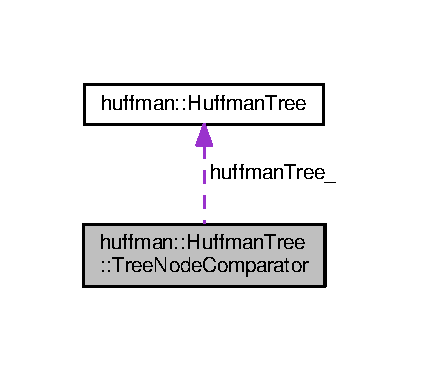
\includegraphics[width=202pt]{structhuffman_1_1HuffmanTree_1_1TreeNodeComparator__coll__graph}
\end{center}
\end{figure}
\subsection*{Public Member Functions}
\begin{DoxyCompactItemize}
\item 
\hyperlink{structhuffman_1_1HuffmanTree_1_1TreeNodeComparator_af7a98f1e7a01c6a239c13fc980fb0de7}{Tree\+Node\+Comparator} (const \hyperlink{classhuffman_1_1HuffmanTree}{huffman\+::\+Huffman\+Tree} \&huffman\+Tree)
\item 
bool \hyperlink{structhuffman_1_1HuffmanTree_1_1TreeNodeComparator_a24a7c95bd79dc7e189c2bed39ebece01}{operator()} (const \hyperlink{namespacehuffman_1_1types_a41dc8ca07e19043152b0a5c8b5fec90b}{huffman\+::types\+::handle\+\_\+t} \&a\+Handle, const \hyperlink{namespacehuffman_1_1types_a41dc8ca07e19043152b0a5c8b5fec90b}{huffman\+::types\+::handle\+\_\+t} \&b\+Handle) const 
\end{DoxyCompactItemize}
\subsection*{Public Attributes}
\begin{DoxyCompactItemize}
\item 
const \hyperlink{classhuffman_1_1HuffmanTree}{huffman\+::\+Huffman\+Tree} \& \hyperlink{structhuffman_1_1HuffmanTree_1_1TreeNodeComparator_a2631e58df1a28734ff72d75a68bc9d25}{huffman\+Tree\+\_\+}
\end{DoxyCompactItemize}


\subsection{Detailed Description}
Comparator used for determining order of the nodes when constructing the tree. Nodes are primarily ordered by frequency where lower frequency has higher priority. Nodes are secondarily ordered by the data where smaller data value has higher priority. 

Definition at line 26 of file Huffman\+Tree.\+h.



\subsection{Constructor \& Destructor Documentation}
\index{huffman\+::\+Huffman\+Tree\+::\+Tree\+Node\+Comparator@{huffman\+::\+Huffman\+Tree\+::\+Tree\+Node\+Comparator}!Tree\+Node\+Comparator@{Tree\+Node\+Comparator}}
\index{Tree\+Node\+Comparator@{Tree\+Node\+Comparator}!huffman\+::\+Huffman\+Tree\+::\+Tree\+Node\+Comparator@{huffman\+::\+Huffman\+Tree\+::\+Tree\+Node\+Comparator}}
\subsubsection[{\texorpdfstring{Tree\+Node\+Comparator(const huffman\+::\+Huffman\+Tree \&huffman\+Tree)}{TreeNodeComparator(const huffman::HuffmanTree &huffmanTree)}}]{\setlength{\rightskip}{0pt plus 5cm}huffman\+::\+Huffman\+Tree\+::\+Tree\+Node\+Comparator\+::\+Tree\+Node\+Comparator (
\begin{DoxyParamCaption}
\item[{const {\bf huffman\+::\+Huffman\+Tree} \&}]{huffman\+Tree}
\end{DoxyParamCaption}
)\hspace{0.3cm}{\ttfamily [inline]}}\hypertarget{structhuffman_1_1HuffmanTree_1_1TreeNodeComparator_af7a98f1e7a01c6a239c13fc980fb0de7}{}\label{structhuffman_1_1HuffmanTree_1_1TreeNodeComparator_af7a98f1e7a01c6a239c13fc980fb0de7}


Definition at line 28 of file Huffman\+Tree.\+h.



\subsection{Member Function Documentation}
\index{huffman\+::\+Huffman\+Tree\+::\+Tree\+Node\+Comparator@{huffman\+::\+Huffman\+Tree\+::\+Tree\+Node\+Comparator}!operator()@{operator()}}
\index{operator()@{operator()}!huffman\+::\+Huffman\+Tree\+::\+Tree\+Node\+Comparator@{huffman\+::\+Huffman\+Tree\+::\+Tree\+Node\+Comparator}}
\subsubsection[{\texorpdfstring{operator()(const huffman\+::types\+::handle\+\_\+t \&a\+Handle, const huffman\+::types\+::handle\+\_\+t \&b\+Handle) const }{operator()(const huffman::types::handle_t &aHandle, const huffman::types::handle_t &bHandle) const }}]{\setlength{\rightskip}{0pt plus 5cm}bool huffman\+::\+Huffman\+Tree\+::\+Tree\+Node\+Comparator\+::operator() (
\begin{DoxyParamCaption}
\item[{const {\bf huffman\+::types\+::handle\+\_\+t} \&}]{a\+Handle, }
\item[{const {\bf huffman\+::types\+::handle\+\_\+t} \&}]{b\+Handle}
\end{DoxyParamCaption}
) const}\hypertarget{structhuffman_1_1HuffmanTree_1_1TreeNodeComparator_a24a7c95bd79dc7e189c2bed39ebece01}{}\label{structhuffman_1_1HuffmanTree_1_1TreeNodeComparator_a24a7c95bd79dc7e189c2bed39ebece01}


Definition at line 198 of file Huffman\+Tree.\+cpp.



\subsection{Member Data Documentation}
\index{huffman\+::\+Huffman\+Tree\+::\+Tree\+Node\+Comparator@{huffman\+::\+Huffman\+Tree\+::\+Tree\+Node\+Comparator}!huffman\+Tree\+\_\+@{huffman\+Tree\+\_\+}}
\index{huffman\+Tree\+\_\+@{huffman\+Tree\+\_\+}!huffman\+::\+Huffman\+Tree\+::\+Tree\+Node\+Comparator@{huffman\+::\+Huffman\+Tree\+::\+Tree\+Node\+Comparator}}
\subsubsection[{\texorpdfstring{huffman\+Tree\+\_\+}{huffmanTree_}}]{\setlength{\rightskip}{0pt plus 5cm}const {\bf huffman\+::\+Huffman\+Tree}\& huffman\+::\+Huffman\+Tree\+::\+Tree\+Node\+Comparator\+::huffman\+Tree\+\_\+}\hypertarget{structhuffman_1_1HuffmanTree_1_1TreeNodeComparator_a2631e58df1a28734ff72d75a68bc9d25}{}\label{structhuffman_1_1HuffmanTree_1_1TreeNodeComparator_a2631e58df1a28734ff72d75a68bc9d25}


Definition at line 33 of file Huffman\+Tree.\+h.



The documentation for this struct was generated from the following files\+:\begin{DoxyCompactItemize}
\item 
\hyperlink{HuffmanTree_8h}{Huffman\+Tree.\+h}\item 
\hyperlink{HuffmanTree_8cpp}{Huffman\+Tree.\+cpp}\end{DoxyCompactItemize}

\chapter{File Documentation}
\hypertarget{BitStack_8cpp}{}\section{Bit\+Stack.\+cpp File Reference}
\label{BitStack_8cpp}\index{Bit\+Stack.\+cpp@{Bit\+Stack.\+cpp}}
{\ttfamily \#include \char`\"{}Bit\+Stack.\+h\char`\"{}}\\*
Include dependency graph for Bit\+Stack.\+cpp\+:
\nopagebreak
\begin{figure}[H]
\begin{center}
\leavevmode
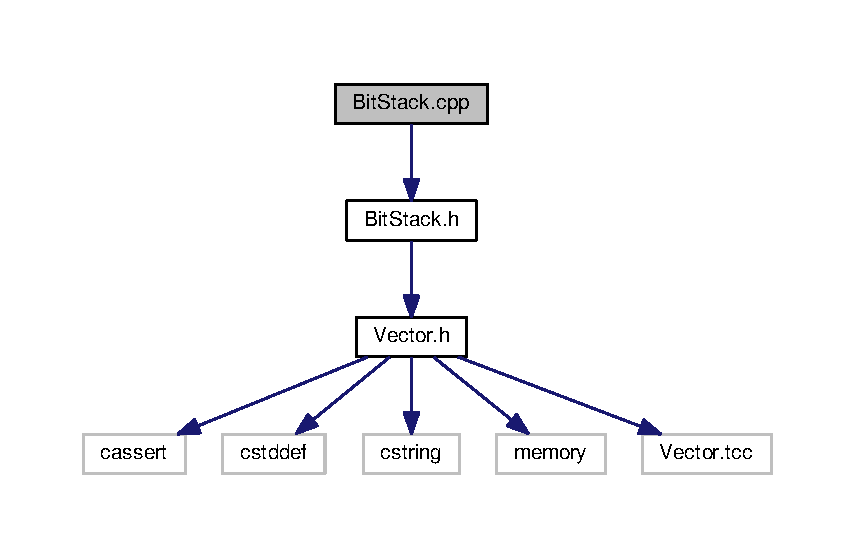
\includegraphics[width=350pt]{BitStack_8cpp__incl}
\end{center}
\end{figure}

\hypertarget{BitStack_8h}{}\section{Bit\+Stack.\+h File Reference}
\label{BitStack_8h}\index{Bit\+Stack.\+h@{Bit\+Stack.\+h}}
{\ttfamily \#include \char`\"{}Vector.\+h\char`\"{}}\\*
Include dependency graph for Bit\+Stack.\+h\+:
\nopagebreak
\begin{figure}[H]
\begin{center}
\leavevmode
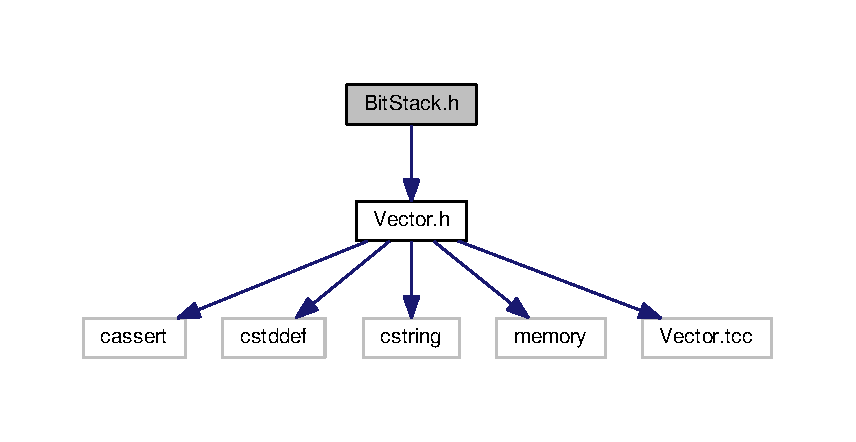
\includegraphics[width=350pt]{BitStack_8h__incl}
\end{center}
\end{figure}
This graph shows which files directly or indirectly include this file\+:
\nopagebreak
\begin{figure}[H]
\begin{center}
\leavevmode
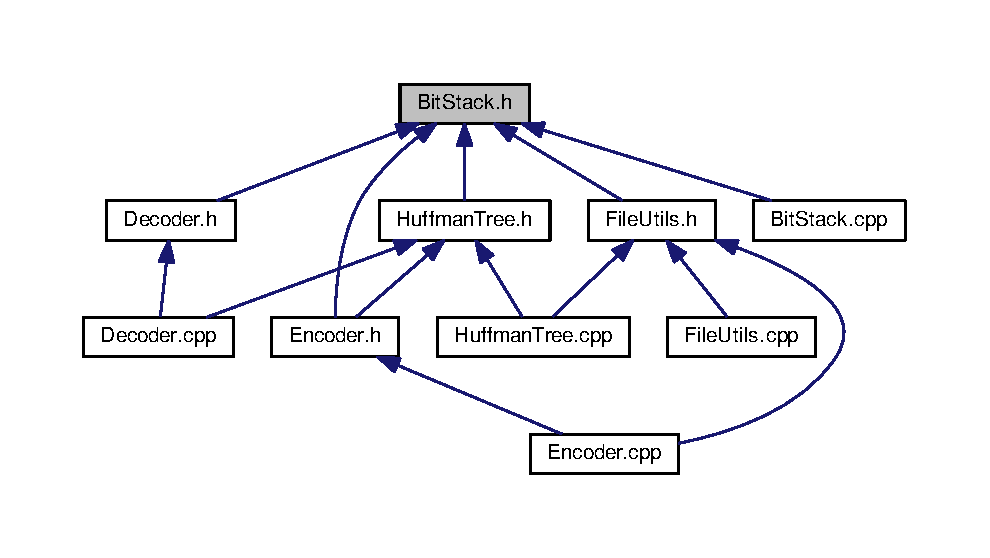
\includegraphics[width=350pt]{BitStack_8h__dep__incl}
\end{center}
\end{figure}
\subsection*{Classes}
\begin{DoxyCompactItemize}
\item 
class \hyperlink{classcommon_1_1BitStack}{common\+::\+Bit\+Stack}
\end{DoxyCompactItemize}
\subsection*{Namespaces}
\begin{DoxyCompactItemize}
\item 
 \hyperlink{namespacecommon}{common}
\end{DoxyCompactItemize}

\hypertarget{huffman_2CMakeLists_8txt}{}\section{C\+Make\+Lists.\+txt File Reference}
\label{huffman_2CMakeLists_8txt}\index{C\+Make\+Lists.\+txt@{C\+Make\+Lists.\+txt}}
\subsection*{Functions}
\begin{DoxyCompactItemize}
\item 
\hyperlink{huffman_2CMakeLists_8txt_a2b52eb823cda5c59fd980aeb6c0cc18f}{project} (Huffman) set(huffman\+\_\+source\+\_\+files Huffman\+Tree.\+cpp Tree\+Node.\+cpp io/File\+Utils.\+cpp Common.\+h Encoder.\+cpp Decoder.\+cpp) include\+\_\+directories(\$
\end{DoxyCompactItemize}


\subsection{Function Documentation}
\index{huffman/\+C\+Make\+Lists.\+txt@{huffman/\+C\+Make\+Lists.\+txt}!project@{project}}
\index{project@{project}!huffman/\+C\+Make\+Lists.\+txt@{huffman/\+C\+Make\+Lists.\+txt}}
\subsubsection[{\texorpdfstring{project(\+Huffman) set(huffman\+\_\+source\+\_\+files Huffman\+Tree.\+cpp Tree\+Node.\+cpp io/\+File\+Utils.\+cpp Common.\+h Encoder.\+cpp Decoder.\+cpp) include\+\_\+directories(\$}{project(Huffman) set(huffman_source_files HuffmanTree.cpp TreeNode.cpp io/FileUtils.cpp Common.h Encoder.cpp Decoder.cpp) include_directories($}}]{\setlength{\rightskip}{0pt plus 5cm}project (
\begin{DoxyParamCaption}
\item[{Huffman}]{}
\end{DoxyParamCaption}
)}\hypertarget{huffman_2CMakeLists_8txt_a2b52eb823cda5c59fd980aeb6c0cc18f}{}\label{huffman_2CMakeLists_8txt_a2b52eb823cda5c59fd980aeb6c0cc18f}


Definition at line 1 of file huffman/\+C\+Make\+Lists.\+txt.


\hypertarget{common_2CMakeLists_8txt}{}\section{C\+Make\+Lists.\+txt File Reference}
\label{common_2CMakeLists_8txt}\index{C\+Make\+Lists.\+txt@{C\+Make\+Lists.\+txt}}
\subsection*{Functions}
\begin{DoxyCompactItemize}
\item 
\hyperlink{common_2CMakeLists_8txt_a45df9617f6fc7e1d4b30dba2c29d3dd6}{project} (Common) set(common\+\_\+source\+\_\+files Vector.\+h Bit\+Stack.\+cpp Bit\+Stack.\+h) add\+\_\+library(Common \$
\end{DoxyCompactItemize}


\subsection{Function Documentation}
\index{common/\+C\+Make\+Lists.\+txt@{common/\+C\+Make\+Lists.\+txt}!project@{project}}
\index{project@{project}!common/\+C\+Make\+Lists.\+txt@{common/\+C\+Make\+Lists.\+txt}}
\subsubsection[{\texorpdfstring{project(\+Common) set(common\+\_\+source\+\_\+files Vector.\+h Bit\+Stack.\+cpp Bit\+Stack.\+h) add\+\_\+library(\+Common \$}{project(Common) set(common_source_files Vector.h BitStack.cpp BitStack.h) add_library(Common $}}]{\setlength{\rightskip}{0pt plus 5cm}project (
\begin{DoxyParamCaption}
\item[{Common}]{}
\end{DoxyParamCaption}
)}\hypertarget{common_2CMakeLists_8txt_a45df9617f6fc7e1d4b30dba2c29d3dd6}{}\label{common_2CMakeLists_8txt_a45df9617f6fc7e1d4b30dba2c29d3dd6}


Definition at line 1 of file common/\+C\+Make\+Lists.\+txt.


\hypertarget{Common_8h}{}\section{Common.\+h File Reference}
\label{Common_8h}\index{Common.\+h@{Common.\+h}}
{\ttfamily \#include $<$array$>$}\\*
Include dependency graph for Common.\+h\+:\nopagebreak
\begin{figure}[H]
\begin{center}
\leavevmode
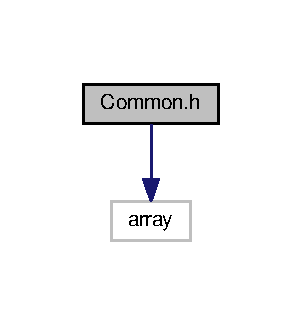
\includegraphics[width=145pt]{Common_8h__incl}
\end{center}
\end{figure}
This graph shows which files directly or indirectly include this file\+:
\nopagebreak
\begin{figure}[H]
\begin{center}
\leavevmode
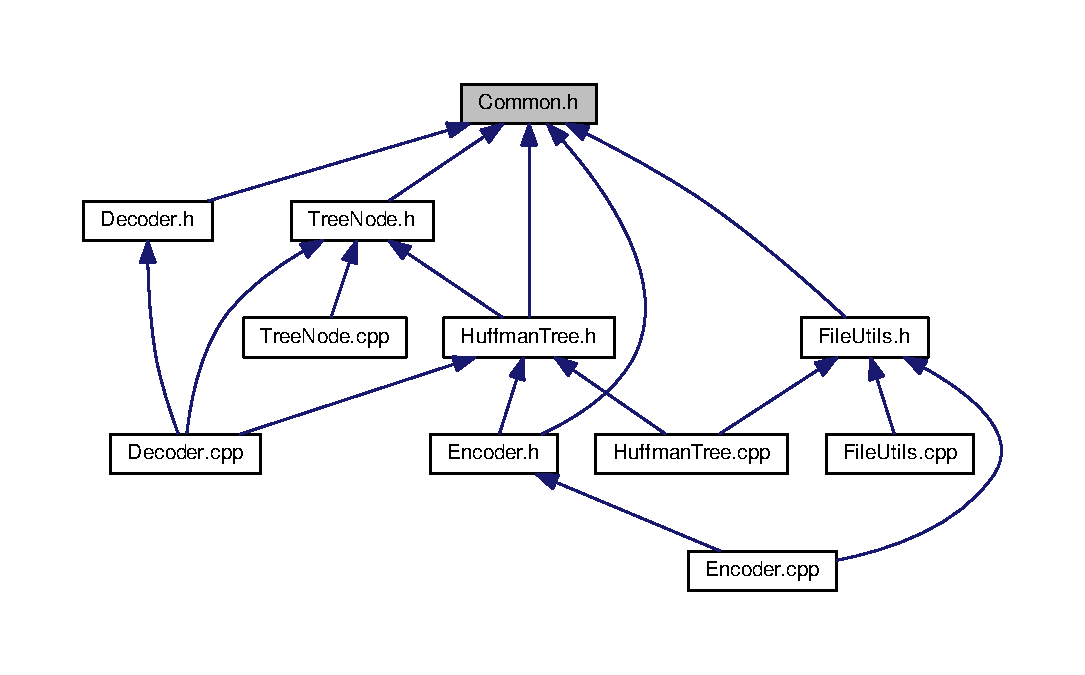
\includegraphics[width=350pt]{Common_8h__dep__incl}
\end{center}
\end{figure}
\subsection*{Namespaces}
\begin{DoxyCompactItemize}
\item 
 \hyperlink{namespacehuffman}{huffman}
\item 
 \hyperlink{namespacehuffman_1_1constants}{huffman\+::constants}
\item 
 \hyperlink{namespacehuffman_1_1types}{huffman\+::types}
\end{DoxyCompactItemize}
\subsection*{Typedefs}
\begin{DoxyCompactItemize}
\item 
using \hyperlink{namespacehuffman_1_1types_a562530b9038f6a3cb2923f1c116a450c}{huffman\+::types\+::encode\+\_\+entry\+\_\+t} = std\+::pair$<$ uint32\+\_\+t, uint8\+\_\+t $>$
\item 
using \hyperlink{namespacehuffman_1_1types_a2d111e21190970dfeb935ef0786973c0}{huffman\+::types\+::encode\+\_\+table\+\_\+t} = std\+::array$<$ encode\+\_\+entry\+\_\+t, constants\+::\+C\+H\+A\+R\+A\+C\+T\+E\+RS $>$
\item 
using \hyperlink{namespacehuffman_1_1types_a41dc8ca07e19043152b0a5c8b5fec90b}{huffman\+::types\+::handle\+\_\+t} = int
\item 
using \hyperlink{namespacehuffman_1_1types_a198fb2bbef1012ab1696124836c56f0d}{huffman\+::types\+::byte\+\_\+t} = unsigned char
\end{DoxyCompactItemize}
\subsection*{Variables}
\begin{DoxyCompactItemize}
\item 
constexpr unsigned \hyperlink{namespacehuffman_1_1constants_a263e0c34ff9ba6afe32efbc1eeabdf88}{huffman\+::constants\+::\+C\+H\+A\+R\+A\+C\+T\+E\+RS} = 256
\item 
constexpr unsigned \hyperlink{namespacehuffman_1_1constants_a9bbdd97bbc9095087fd624645d1082fe}{huffman\+::constants\+::\+M\+A\+X\+\_\+\+C\+O\+D\+E\+\_\+\+L\+E\+N\+G\+TH} = 32
\item 
static constexpr unsigned char \hyperlink{namespacehuffman_1_1constants_a89cadeae06b1c8968a40bbde1e1929b6}{huffman\+::constants\+::\+B\+I\+T\+S\+\_\+\+I\+N\+\_\+\+B\+Y\+TE} = 8
\item 
static constexpr int \hyperlink{namespacehuffman_1_1constants_a807803821447a0285e3dfd195ee698e7}{huffman\+::constants\+::empty\+\_\+handle} = -\/1
\end{DoxyCompactItemize}

\hypertarget{Decoder_8cpp}{}\section{Decoder.\+cpp File Reference}
\label{Decoder_8cpp}\index{Decoder.\+cpp@{Decoder.\+cpp}}
{\ttfamily \#include \char`\"{}Decoder.\+h\char`\"{}}\\*
{\ttfamily \#include \char`\"{}Tree\+Node.\+h\char`\"{}}\\*
{\ttfamily \#include \char`\"{}Huffman\+Tree.\+h\char`\"{}}\\*
Include dependency graph for Decoder.\+cpp\+:
\nopagebreak
\begin{figure}[H]
\begin{center}
\leavevmode
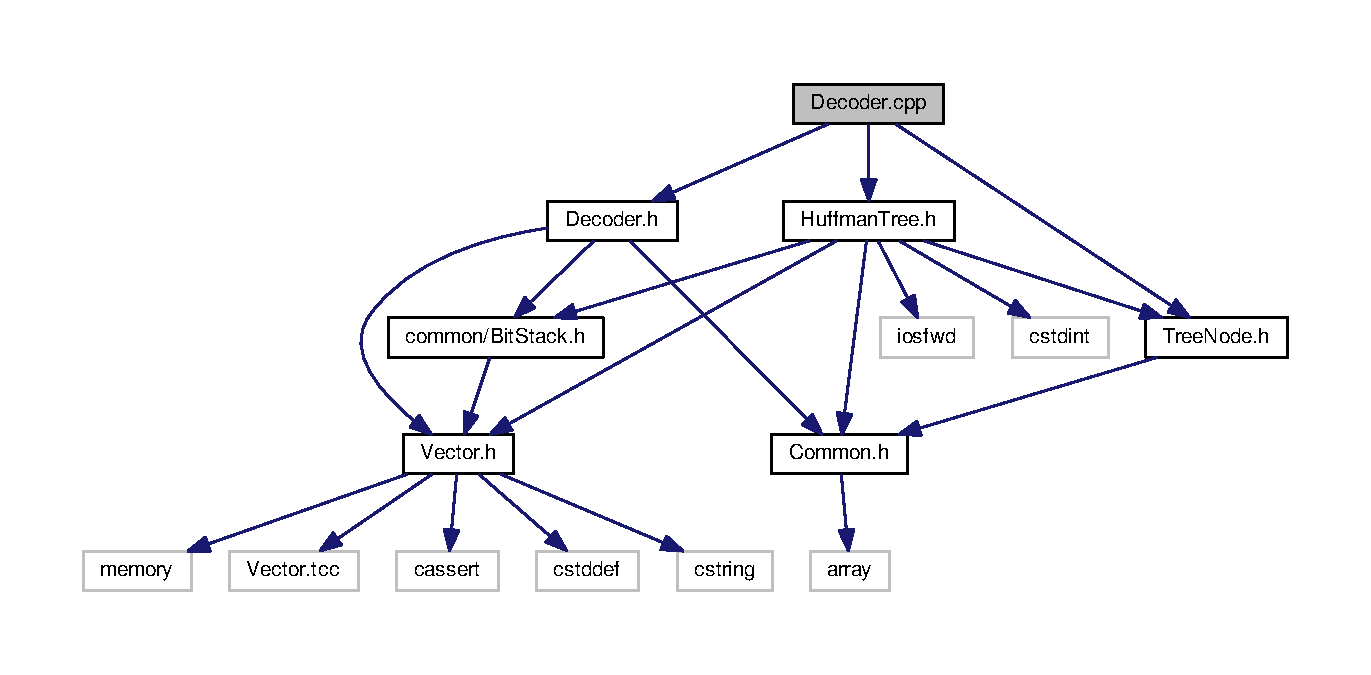
\includegraphics[width=350pt]{Decoder_8cpp__incl}
\end{center}
\end{figure}

\hypertarget{Decoder_8h}{}\section{Decoder.\+h File Reference}
\label{Decoder_8h}\index{Decoder.\+h@{Decoder.\+h}}
{\ttfamily \#include \char`\"{}Bit\+Stack.\+h\char`\"{}}\\*
{\ttfamily \#include \char`\"{}Vector.\+h\char`\"{}}\\*
{\ttfamily \#include \char`\"{}Common.\+h\char`\"{}}\\*
Include dependency graph for Decoder.\+h\+:\nopagebreak
\begin{figure}[H]
\begin{center}
\leavevmode
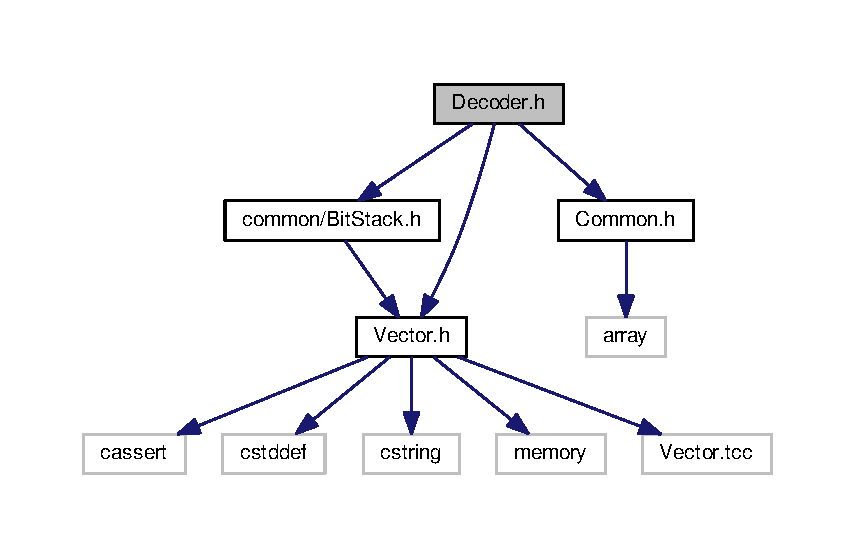
\includegraphics[width=350pt]{Decoder_8h__incl}
\end{center}
\end{figure}
This graph shows which files directly or indirectly include this file\+:\nopagebreak
\begin{figure}[H]
\begin{center}
\leavevmode
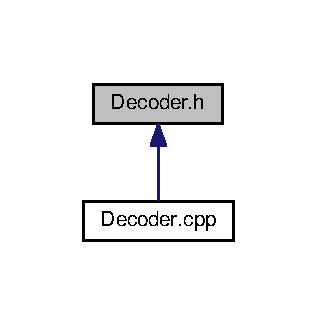
\includegraphics[width=152pt]{Decoder_8h__dep__incl}
\end{center}
\end{figure}
\subsection*{Classes}
\begin{DoxyCompactItemize}
\item 
class \hyperlink{classhuffman_1_1Decoder}{huffman\+::\+Decoder}
\end{DoxyCompactItemize}
\subsection*{Namespaces}
\begin{DoxyCompactItemize}
\item 
 \hyperlink{namespacehuffman}{huffman}
\end{DoxyCompactItemize}

\hypertarget{Encoder_8cpp}{}\section{Encoder.\+cpp File Reference}
\label{Encoder_8cpp}\index{Encoder.\+cpp@{Encoder.\+cpp}}
{\ttfamily \#include \char`\"{}Encoder.\+h\char`\"{}}\\*
{\ttfamily \#include $<$cassert$>$}\\*
{\ttfamily \#include \char`\"{}io/\+File\+Utils.\+h\char`\"{}}\\*
Include dependency graph for Encoder.\+cpp\+:
\nopagebreak
\begin{figure}[H]
\begin{center}
\leavevmode
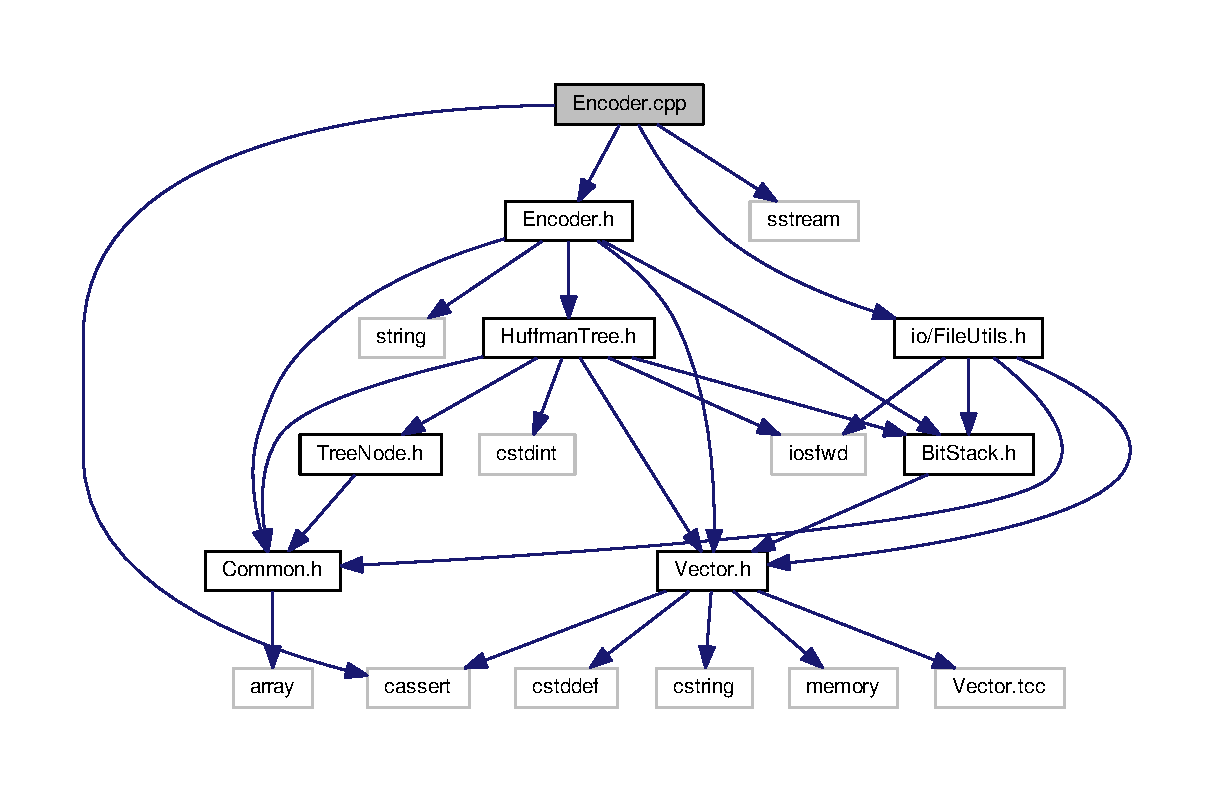
\includegraphics[width=350pt]{Encoder_8cpp__incl}
\end{center}
\end{figure}

\hypertarget{Encoder_8h}{}\section{Encoder.\+h File Reference}
\label{Encoder_8h}\index{Encoder.\+h@{Encoder.\+h}}
{\ttfamily \#include $<$string$>$}\\*
{\ttfamily \#include \char`\"{}common/\+Bit\+Stack.\+h\char`\"{}}\\*
{\ttfamily \#include \char`\"{}common/\+Vector.\+h\char`\"{}}\\*
{\ttfamily \#include \char`\"{}Common.\+h\char`\"{}}\\*
{\ttfamily \#include \char`\"{}Huffman\+Tree.\+h\char`\"{}}\\*
Include dependency graph for Encoder.\+h\+:
\nopagebreak
\begin{figure}[H]
\begin{center}
\leavevmode
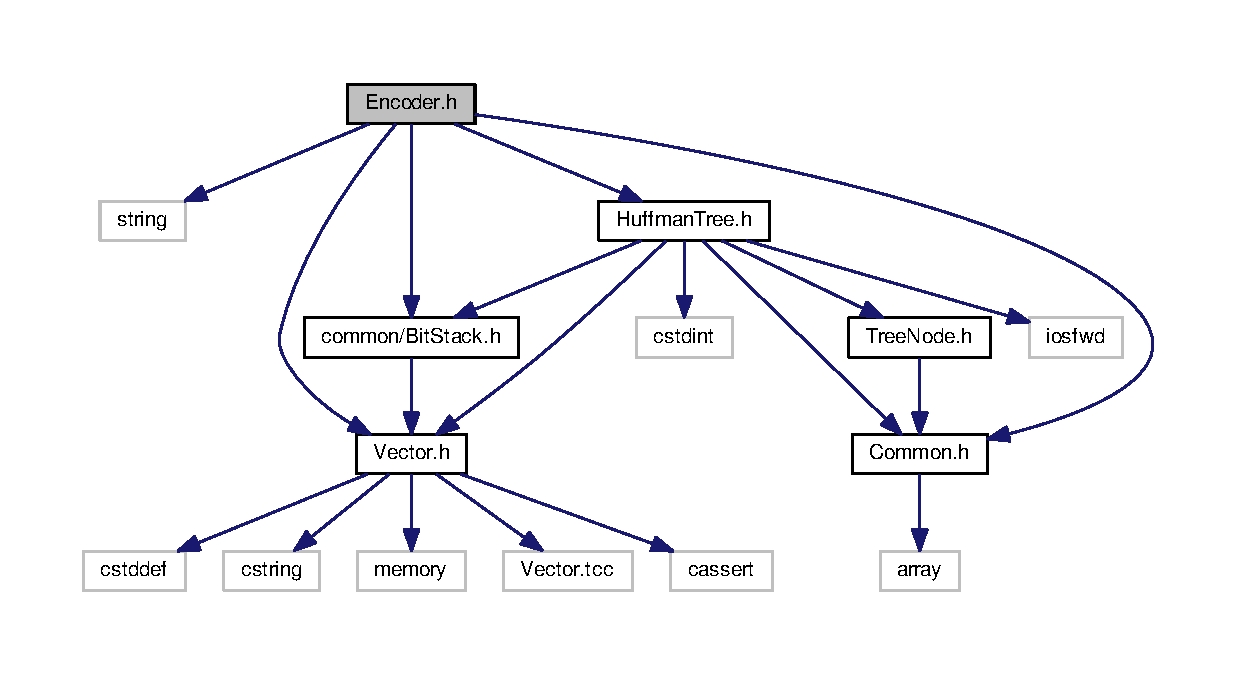
\includegraphics[width=350pt]{Encoder_8h__incl}
\end{center}
\end{figure}
This graph shows which files directly or indirectly include this file\+:
\nopagebreak
\begin{figure}[H]
\begin{center}
\leavevmode
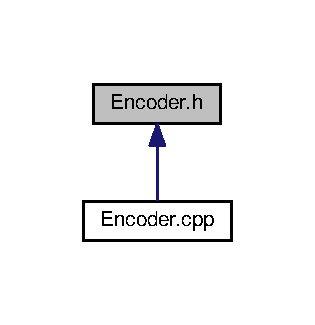
\includegraphics[width=151pt]{Encoder_8h__dep__incl}
\end{center}
\end{figure}
\subsection*{Classes}
\begin{DoxyCompactItemize}
\item 
class \hyperlink{classhuffman_1_1Encoder}{huffman\+::\+Encoder}
\end{DoxyCompactItemize}
\subsection*{Namespaces}
\begin{DoxyCompactItemize}
\item 
 \hyperlink{namespacehuffman}{huffman}
\end{DoxyCompactItemize}

\hypertarget{FileUtils_8cpp}{}\section{File\+Utils.\+cpp File Reference}
\label{FileUtils_8cpp}\index{File\+Utils.\+cpp@{File\+Utils.\+cpp}}
{\ttfamily \#include \char`\"{}File\+Utils.\+h\char`\"{}}\\*
{\ttfamily \#include $<$fstream$>$}\\*
{\ttfamily \#include $<$cassert$>$}\\*
Include dependency graph for File\+Utils.\+cpp\+:
\nopagebreak
\begin{figure}[H]
\begin{center}
\leavevmode
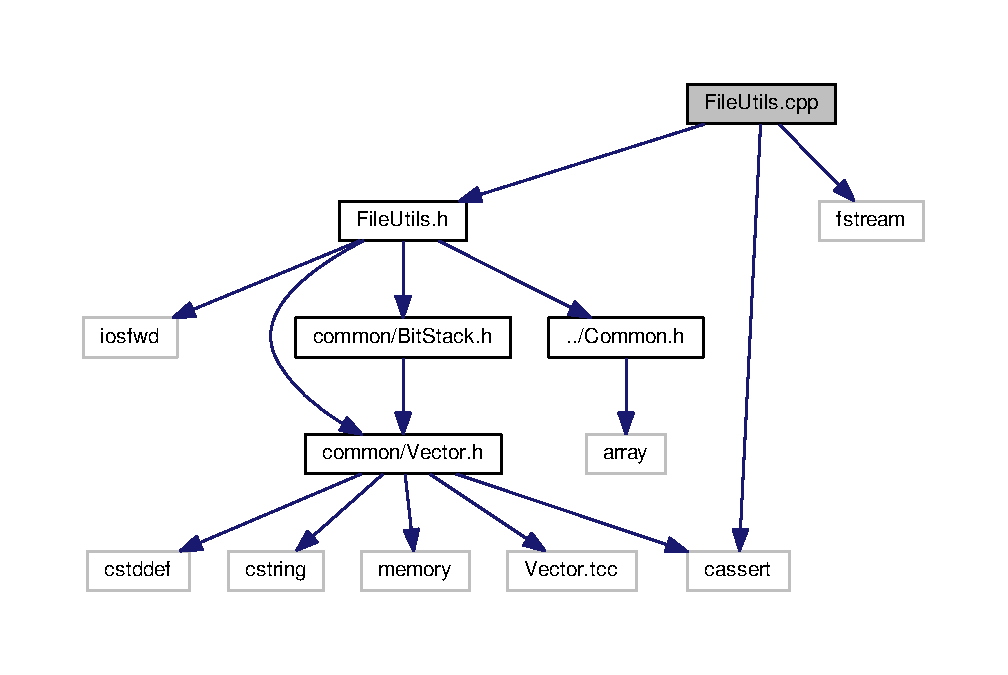
\includegraphics[width=350pt]{FileUtils_8cpp__incl}
\end{center}
\end{figure}
\subsection*{Macros}
\begin{DoxyCompactItemize}
\item 
\#define \hyperlink{FileUtils_8cpp_a7b2104fa9d29c805faf9002be349cf9e}{D\+A\+T\+A\+\_\+\+S\+I\+ZE}(size\+\_\+in\+\_\+bits)~(size\+\_\+in\+\_\+bits + (32 -\/ (size\+\_\+in\+\_\+bits \% 32))) / 8
\end{DoxyCompactItemize}


\subsection{Macro Definition Documentation}
\index{File\+Utils.\+cpp@{File\+Utils.\+cpp}!D\+A\+T\+A\+\_\+\+S\+I\+ZE@{D\+A\+T\+A\+\_\+\+S\+I\+ZE}}
\index{D\+A\+T\+A\+\_\+\+S\+I\+ZE@{D\+A\+T\+A\+\_\+\+S\+I\+ZE}!File\+Utils.\+cpp@{File\+Utils.\+cpp}}
\subsubsection[{\texorpdfstring{D\+A\+T\+A\+\_\+\+S\+I\+ZE}{DATA_SIZE}}]{\setlength{\rightskip}{0pt plus 5cm}\#define D\+A\+T\+A\+\_\+\+S\+I\+ZE(
\begin{DoxyParamCaption}
\item[{}]{size\+\_\+in\+\_\+bits}
\end{DoxyParamCaption}
)~(size\+\_\+in\+\_\+bits + (32 -\/ (size\+\_\+in\+\_\+bits \% 32))) / 8}\hypertarget{FileUtils_8cpp_a7b2104fa9d29c805faf9002be349cf9e}{}\label{FileUtils_8cpp_a7b2104fa9d29c805faf9002be349cf9e}


Definition at line 6 of file File\+Utils.\+cpp.


\hypertarget{FileUtils_8h}{}\section{File\+Utils.\+h File Reference}
\label{FileUtils_8h}\index{File\+Utils.\+h@{File\+Utils.\+h}}
{\ttfamily \#include $<$iosfwd$>$}\\*
{\ttfamily \#include \char`\"{}common/\+Vector.\+h\char`\"{}}\\*
{\ttfamily \#include \char`\"{}common/\+Bit\+Stack.\+h\char`\"{}}\\*
{\ttfamily \#include \char`\"{}../\+Common.\+h\char`\"{}}\\*
Include dependency graph for File\+Utils.\+h\+:
\nopagebreak
\begin{figure}[H]
\begin{center}
\leavevmode
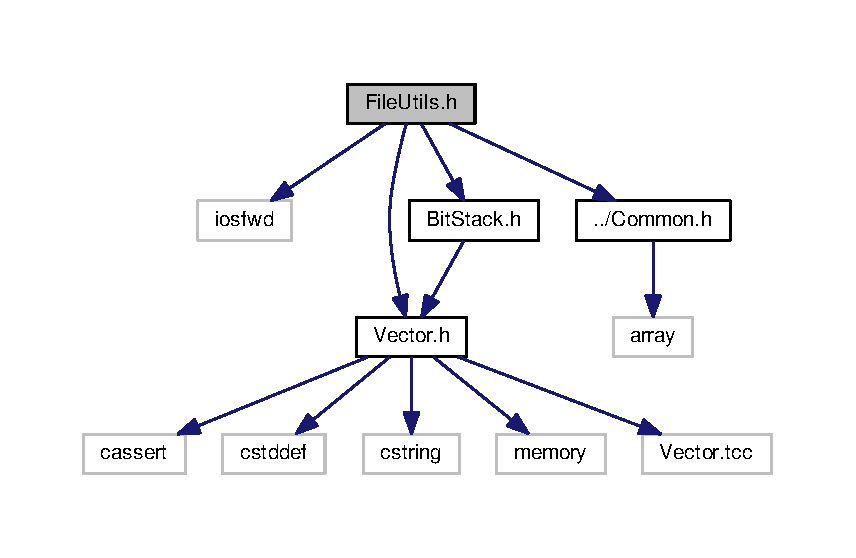
\includegraphics[width=350pt]{FileUtils_8h__incl}
\end{center}
\end{figure}
This graph shows which files directly or indirectly include this file\+:
\nopagebreak
\begin{figure}[H]
\begin{center}
\leavevmode
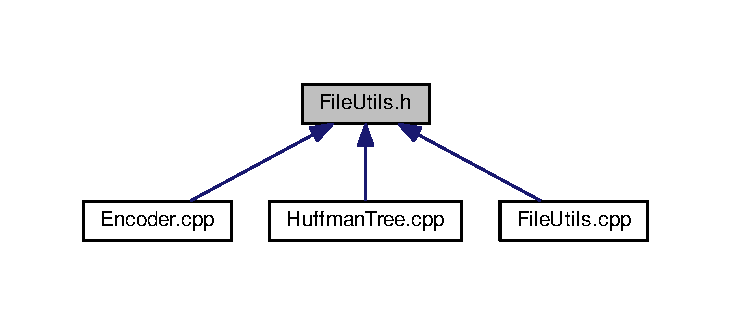
\includegraphics[width=350pt]{FileUtils_8h__dep__incl}
\end{center}
\end{figure}
\subsection*{Namespaces}
\begin{DoxyCompactItemize}
\item 
 \hyperlink{namespacehuffman}{huffman}
\item 
 \hyperlink{namespacehuffman_1_1io}{huffman\+::io}
\end{DoxyCompactItemize}
\subsection*{Functions}
\begin{DoxyCompactItemize}
\item 
common\+::\+Vector$<$ \hyperlink{namespacehuffman_1_1types_a198fb2bbef1012ab1696124836c56f0d}{huffman\+::types\+::byte\+\_\+t} $>$ \hyperlink{namespacehuffman_1_1io_a3dc9d3bd379dd95a993bff408092514a}{huffman\+::io\+::read\+File} (std\+::istream \&istream)
\item 
void \hyperlink{namespacehuffman_1_1io_a46774d6debc0d1318c44db613a700ab0}{huffman\+::io\+::write\+File} (std\+::ostream \&ostream, const common\+::\+Vector$<$ \hyperlink{namespacehuffman_1_1types_a198fb2bbef1012ab1696124836c56f0d}{huffman\+::types\+::byte\+\_\+t} $>$ \&data)
\item 
void \hyperlink{namespacehuffman_1_1io_afa4a671ca46f3b2fdb8052639340178f}{huffman\+::io\+::write\+Binary\+File} (std\+::ostream \&ostream, const \hyperlink{classcommon_1_1BitStack}{common\+::\+Bit\+Stack} \&data, bool magic\+Number=false)
\item 
\hyperlink{classcommon_1_1BitStack}{common\+::\+Bit\+Stack} \hyperlink{namespacehuffman_1_1io_ada2a069d00c22f9fed6aab608d863276}{huffman\+::io\+::read\+Binary\+File} (std\+::istream \&istream, bool ignore\+Header)
\item 
uint64\+\_\+t \hyperlink{namespacehuffman_1_1io_aab7992b4b13288b7ea2a4a1f741f7d65}{huffman\+::io\+::read\+Uint64} (std\+::istream \&istream)
\item 
void \hyperlink{namespacehuffman_1_1io_af709b79bf385345e28dc5e3068fc744a}{huffman\+::io\+::write\+Uint64} (uint64\+\_\+t number, std\+::ostream \&ostream)
\item 
void \hyperlink{namespacehuffman_1_1io_ada1e15818c5ab806b890ad58a7c58270}{huffman\+::io\+::insert\+Byte} (\hyperlink{namespacehuffman_1_1types_a198fb2bbef1012ab1696124836c56f0d}{huffman\+::types\+::byte\+\_\+t} byte, \hyperlink{classcommon_1_1BitStack}{common\+::\+Bit\+Stack} \&vector)
\item 
\hyperlink{namespacehuffman_1_1types_a198fb2bbef1012ab1696124836c56f0d}{huffman\+::types\+::byte\+\_\+t} \hyperlink{namespacehuffman_1_1io_af34a00787e1294fb7b72c7d02d214875}{huffman\+::io\+::read\+Byte} (const \hyperlink{classcommon_1_1BitStack}{common\+::\+Bit\+Stack} \&vector, uint64\+\_\+t start)
\item 
bool \hyperlink{namespacehuffman_1_1io_a3672cf6420fd059c8d726e129c7a1e1f}{huffman\+::io\+::verify\+Magic\+Number} (std\+::istream \&istream)
\item 
void \hyperlink{namespacehuffman_1_1io_a0dcd66b464011e749fd3d8d7d889c529}{huffman\+::io\+::write\+Magic\+Number} (std\+::ostream \&ostream)
\end{DoxyCompactItemize}

\hypertarget{HuffmanTree_8cpp}{}\section{Huffman\+Tree.\+cpp File Reference}
\label{HuffmanTree_8cpp}\index{Huffman\+Tree.\+cpp@{Huffman\+Tree.\+cpp}}
{\ttfamily \#include \char`\"{}Huffman\+Tree.\+h\char`\"{}}\\*
{\ttfamily \#include $<$ostream$>$}\\*
{\ttfamily \#include $<$cassert$>$}\\*
{\ttfamily \#include \char`\"{}io/\+File\+Utils.\+h\char`\"{}}\\*
{\ttfamily \#include \char`\"{}common/\+Priority\+Queue.\+h\char`\"{}}\\*
Include dependency graph for Huffman\+Tree.\+cpp\+:
\nopagebreak
\begin{figure}[H]
\begin{center}
\leavevmode
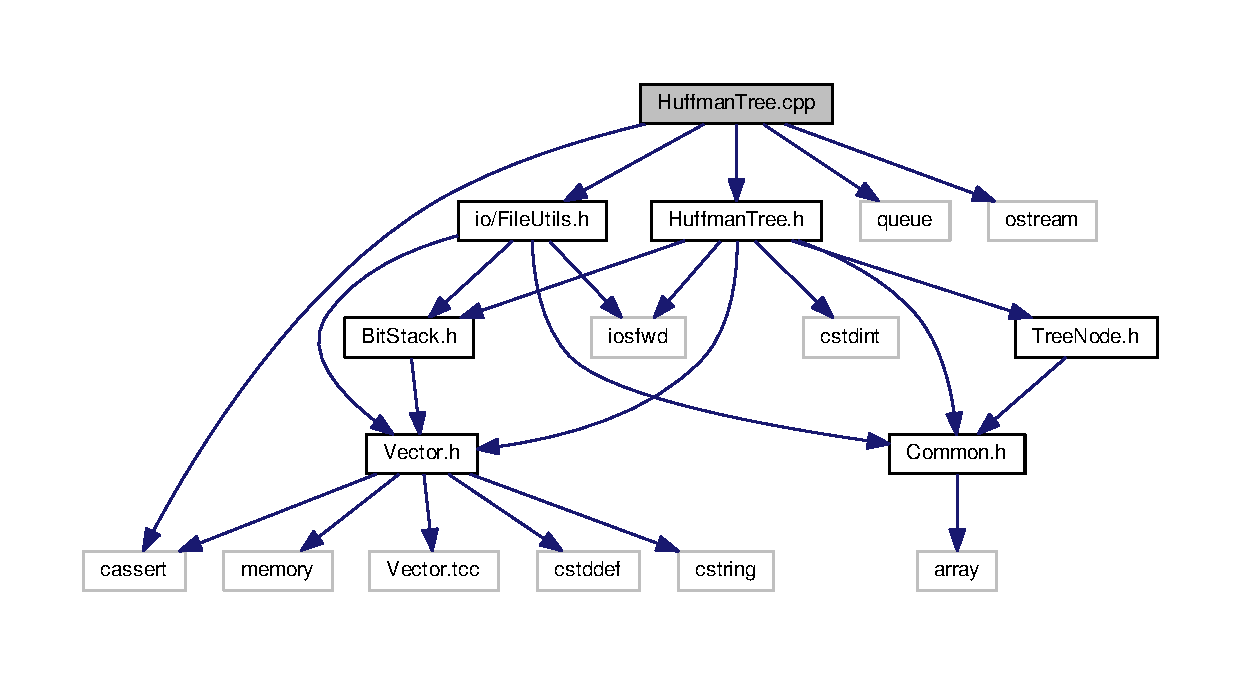
\includegraphics[width=350pt]{HuffmanTree_8cpp__incl}
\end{center}
\end{figure}

\hypertarget{HuffmanTree_8h}{}\section{Huffman\+Tree.\+h File Reference}
\label{HuffmanTree_8h}\index{Huffman\+Tree.\+h@{Huffman\+Tree.\+h}}
{\ttfamily \#include $<$iosfwd$>$}\\*
{\ttfamily \#include $<$cstdint$>$}\\*
{\ttfamily \#include \char`\"{}Vector.\+h\char`\"{}}\\*
{\ttfamily \#include \char`\"{}Bit\+Stack.\+h\char`\"{}}\\*
{\ttfamily \#include \char`\"{}Common.\+h\char`\"{}}\\*
{\ttfamily \#include \char`\"{}Tree\+Node.\+h\char`\"{}}\\*
Include dependency graph for Huffman\+Tree.\+h\+:\nopagebreak
\begin{figure}[H]
\begin{center}
\leavevmode
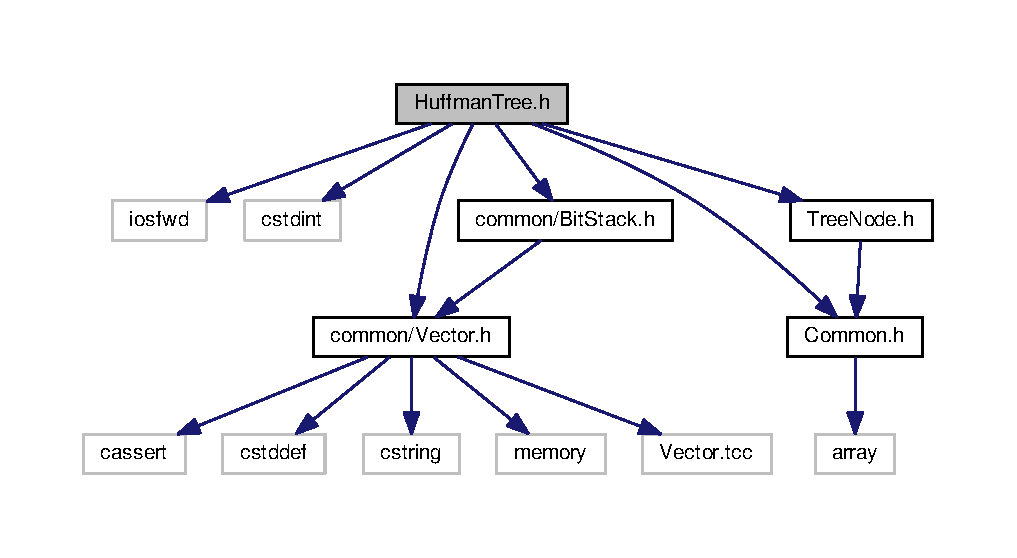
\includegraphics[width=350pt]{HuffmanTree_8h__incl}
\end{center}
\end{figure}
This graph shows which files directly or indirectly include this file\+:\nopagebreak
\begin{figure}[H]
\begin{center}
\leavevmode
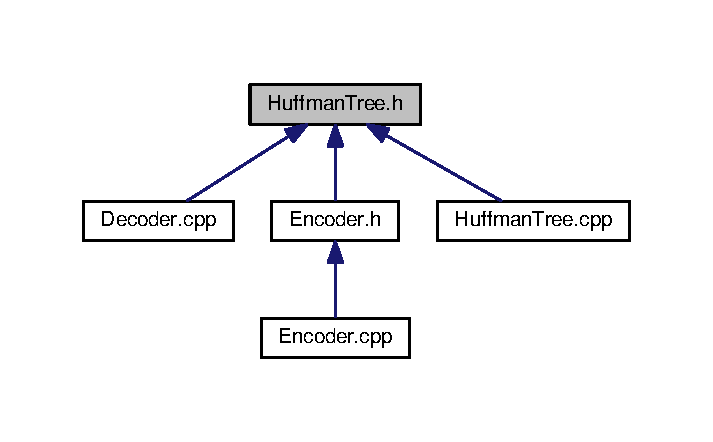
\includegraphics[width=342pt]{HuffmanTree_8h__dep__incl}
\end{center}
\end{figure}
\subsection*{Classes}
\begin{DoxyCompactItemize}
\item 
class \hyperlink{classhuffman_1_1HuffmanTree}{huffman\+::\+Huffman\+Tree}
\item 
struct \hyperlink{structhuffman_1_1HuffmanTree_1_1TreeNodeComparator}{huffman\+::\+Huffman\+Tree\+::\+Tree\+Node\+Comparator}
\end{DoxyCompactItemize}
\subsection*{Namespaces}
\begin{DoxyCompactItemize}
\item 
 \hyperlink{namespacehuffman}{huffman}
\end{DoxyCompactItemize}

\hypertarget{TreeNode_8cpp}{}\section{Tree\+Node.\+cpp File Reference}
\label{TreeNode_8cpp}\index{Tree\+Node.\+cpp@{Tree\+Node.\+cpp}}
{\ttfamily \#include \char`\"{}Tree\+Node.\+h\char`\"{}}\\*
Include dependency graph for Tree\+Node.\+cpp\+:\nopagebreak
\begin{figure}[H]
\begin{center}
\leavevmode
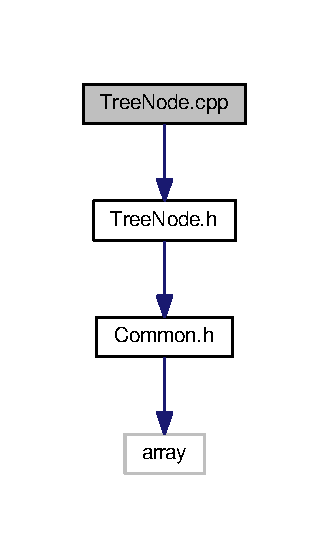
\includegraphics[width=158pt]{TreeNode_8cpp__incl}
\end{center}
\end{figure}

\hypertarget{TreeNode_8h}{}\section{Tree\+Node.\+h File Reference}
\label{TreeNode_8h}\index{Tree\+Node.\+h@{Tree\+Node.\+h}}
{\ttfamily \#include \char`\"{}Common.\+h\char`\"{}}\\*
Include dependency graph for Tree\+Node.\+h\+:
\nopagebreak
\begin{figure}[H]
\begin{center}
\leavevmode
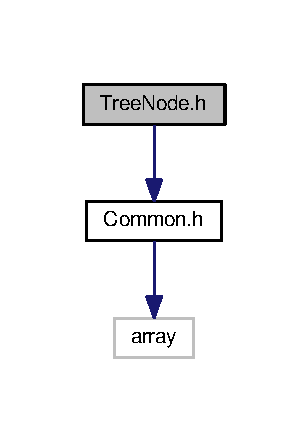
\includegraphics[width=148pt]{TreeNode_8h__incl}
\end{center}
\end{figure}
This graph shows which files directly or indirectly include this file\+:
\nopagebreak
\begin{figure}[H]
\begin{center}
\leavevmode
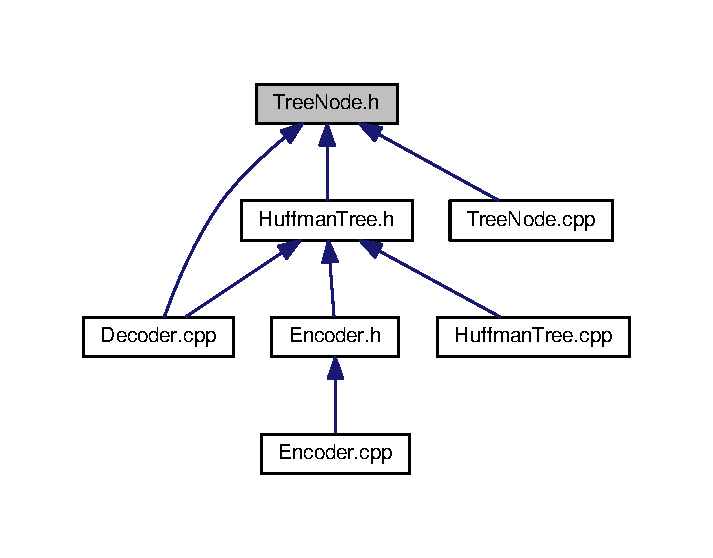
\includegraphics[width=342pt]{TreeNode_8h__dep__incl}
\end{center}
\end{figure}
\subsection*{Classes}
\begin{DoxyCompactItemize}
\item 
class \hyperlink{classhuffman_1_1TreeNode}{huffman\+::\+Tree\+Node}
\end{DoxyCompactItemize}
\subsection*{Namespaces}
\begin{DoxyCompactItemize}
\item 
 \hyperlink{namespacehuffman}{huffman}
\end{DoxyCompactItemize}

\hypertarget{Vector_8h}{}\section{Vector.\+h File Reference}
\label{Vector_8h}\index{Vector.\+h@{Vector.\+h}}
{\ttfamily \#include $<$cassert$>$}\\*
{\ttfamily \#include $<$cstddef$>$}\\*
{\ttfamily \#include $<$cstring$>$}\\*
{\ttfamily \#include $<$memory$>$}\\*
{\ttfamily \#include \char`\"{}Vector.\+tcc\char`\"{}}\\*
Include dependency graph for Vector.\+h\+:
\nopagebreak
\begin{figure}[H]
\begin{center}
\leavevmode
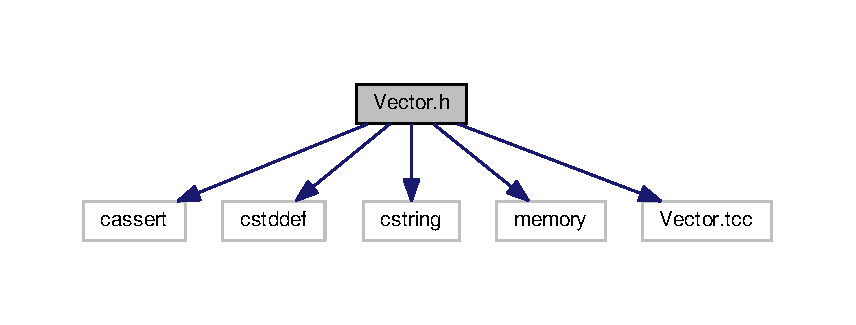
\includegraphics[width=350pt]{Vector_8h__incl}
\end{center}
\end{figure}
This graph shows which files directly or indirectly include this file\+:
\nopagebreak
\begin{figure}[H]
\begin{center}
\leavevmode
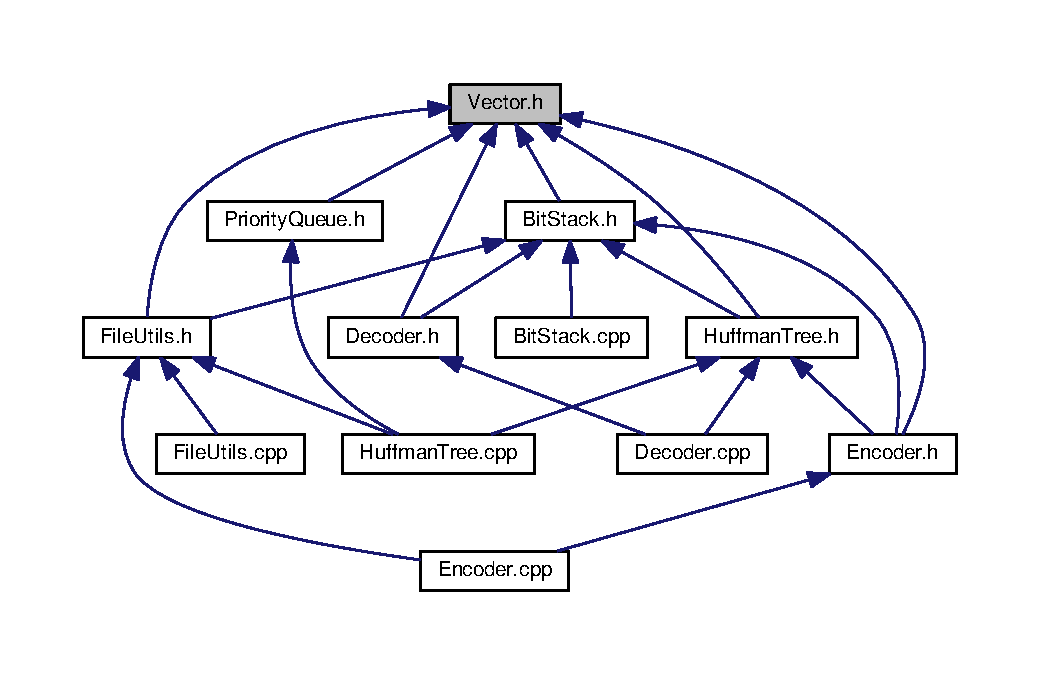
\includegraphics[width=350pt]{Vector_8h__dep__incl}
\end{center}
\end{figure}

%--- End generated contents ---

% Index
\backmatter
\newpage
\phantomsection
\clearemptydoublepage
\addcontentsline{toc}{chapter}{Index}
\printindex

\end{document}
